\documentclass[12pt,oneside]{uhthesis}
\usepackage{subfigure}
\usepackage[ruled,lined,linesnumbered,titlenumbered,algochapter,onelanguage]{algorithm2e}
\usepackage{amsmath}
\usepackage{amssymb}
\usepackage{amsbsy}
\usepackage{caption,booktabs}
\captionsetup{ justification = centering }
%\usepackage{mathpazo}
\usepackage{float}
\setlength{\marginparwidth}{2cm}
\usepackage{todonotes}
\usepackage{listings}
\usepackage{xcolor}
\usepackage{changepage}
\usepackage{multicol}
\usepackage{graphicx}
\usepackage{svg}
\floatstyle{plaintop}
\restylefloat{table}
\addbibresource{Bibliography.bib}
% \setlength{\parskip}{\baselineskip}%
\renewcommand{\tablename}{Tabla}
\renewcommand{\listalgorithmcfname}{Índice de Algoritmos}
%\dontprintsemicolon
\SetAlgoNoEnd
\DeclareUnicodeCharacter{0301}{í}
\definecolor{codegreen}{rgb}{0,0.6,0}
\definecolor{codegray}{rgb}{0.5,0.5,0.5}
\definecolor{codepurple}{rgb}{0.58,0,0.82}
\definecolor{backcolour}{rgb}{0.95,0.95,0.92}

\lstdefinestyle{mystyle}{
    backgroundcolor=\color{backcolour},   
    commentstyle=\color{codegreen},
    keywordstyle=\color{purple},
    numberstyle=\tiny\color{codegray},
    stringstyle=\color{codepurple},
    basicstyle=\ttfamily\footnotesize,
    breakatwhitespace=false,         
    breaklines=true,                 
    captionpos=b,                    
    keepspaces=true,                 
    numbers=left,                    
    numbersep=5pt,                  
    showspaces=false,                
    showstringspaces=false,
    showtabs=false,                  
    tabsize=4
}

\lstset{style=mystyle}

\title{Extracción automática de argumentos en textos de opinión en la prensa cubana}
\author{\\\vspace{0.25cm}Luis Ernesto Ibarra Vázquez}
\advisor{\\\vspace{0.25cm}MSc. Damian Valdés Santiago}
\degree{Licenciado en Ciencia de la Computación}
\faculty{Facultad de Matemática y Computación}
\date{28 de noviembre del 2022\\\vspace{0.25cm}\href{https://github.com/luisoibarra/thesis}{github.com/luisoibarra/thesis}} % TODO PREGUNTA EL repo de la tesis o el de la implementación?
\logo{Graphics/uhlogo}
\makenomenclature

\renewcommand{\vec}[1]{\boldsymbol{#1}}
\newcommand{\diff}[1]{\ensuremath{\mathrm{d}#1}}
\newcommand{\me}[1]{\mathrm{e}^{#1}}
\newcommand{\pf}{\mathfrak{p}}
\newcommand{\qf}{\mathfrak{q}}
%\newcommand{\kf}{\mathfrak{k}}
\newcommand{\kt}{\mathtt{k}}
\newcommand{\mf}{\mathfrak{m}}
\newcommand{\hf}{\mathfrak{h}}
\newcommand{\fac}{\mathrm{fac}}
\newcommand{\maxx}[1]{\max\left\{ #1 \right\} }
\newcommand{\minn}[1]{\min\left\{ #1 \right\} }
\newcommand{\lldpcf}{1.25}
\newcommand{\nnorm}[1]{\left\lvert #1 \right\rvert }
\renewcommand{\lstlistingname}{Ejemplo de código}
\renewcommand{\lstlistlistingname}{Ejemplos de código}

\begin{document}

\frontmatter
\maketitle

\begin{dedication}
A mis amigos y familia, a todas las personas que estuvieron en mi vida dando su apoyo y ayuda para superar los obstáculos.
\end{dedication}
\begin{acknowledgements}
    Agradecimientos
\end{acknowledgements}
\begin{opinion}
La lingüística computacional es una rama multidisciplinaria que procesa grandes 
cantidades de textos escritos. La tesis presentada por Luis Ernesto Ibarra Vázquez 
propone un algoritmo basado en modelos de aprendizaje automático para la segmentación 
y clasificación de enunciados argumentativos en textos de la sección “Cartas a la Dirección” 
del periódico \emph{Granma}.

La tesis se ubica en el marco de un proyecto \emph{Dinámicas sociales, políticas y económicas en el 
discurso público en Cuba de principio del siglo XXI: estudios de CORESPUC}, asociado al Programa 
Nacional de Ciencia y Técnica “Las Ciencias Sociales y las humanidades. Desafíos ante la estrategia 
de desarrollo de la sociedad cubana”, Código PN223LH011-011, Ministerio de Ciencia, Tecnología y 
Medio Ambiente (CITMA), Cuba, 2021-2023.

Por ello, Luis Ernesto tuvo que estudiar la materia referida, que no está incluida en el currículo 
de la carrera y trabajó mostrando creatividad, disciplina, entrega y rigor. Deseo destacar su 
profundización en el estudio computacional de la argumentación y la proposición de soluciones de 
software útiles para el análisis de enunciados argumentativos en español.

La investigación realizada por el estudiante incluyó diversos corpus en idioma inglés con 
diferentes anotaciones de la argumentación que se usaron para el entrenamiento de modelos de 
aprendizaje automático proyectivos para clasificar los enunciados argumentativos en español, a 
partir del conocimiento de la anotación en idioma inglés. Se compararon varios modelos y el mejor 
fue utilizado para la clasificación de enunciados de las Cartas a la Dirección del periódico Granma. 
Este trabajo es un primer paso positivo en el estudio automático de la argumentación de nuestra variante 
del español y llevará una posterior revisión por lingüistas. Dicho corpus anotado será importante para la 
realización de análisis sociolingüísticos del corpus donde la argumentación es una variable de interés para 
el proyecto CORESPUC.

Durante el desarrollo del trabajo, Luis Ernesto demostró habilidades para el trabajo con la bibliografía y 
creatividad para proponer soluciones a problemas de implementación, entre otras competencias de programación 
en el lenguaje Python y sus diversos \emph{frameworks}. Así, se logró cumplir el objetivo de esta tesis.

Por tanto, considero que al estudiante Luis Ernesto Ibarra Vázquez debe otorgársele la máxima calificación 
(5 puntos, Excelente), y estoy seguro que en el futuro Luis Ernesto se desempeñará como un excelente profesional 
de la Ciencia de la Computación.

\begin{flushright}

\includegraphics[scale=0.2]{Graphics/firma_enhanced.jpg}\\
MSc. Damian Valdés Santiago\\
21 de noviembre de 2022    
\end{flushright}

\end{opinion}
\begin{resumen}
% Resumen: IMRD, 250 palabras

% Introducción al problema
%  - Cuál es?
%  - Por qué es importante resolverlo?
% Cómo puede ser o es resuelto?
%  - Qué problemas tiene este proceso?
% Propuesta para mejorar el proceso de resolución del problema
%  - Modelo
%  - Resultados  

El estudio de la argumentación en la prensa cubana es un campo en donde se han reportado
relativamente pocas investigaciones. En estos estudios es posible obtener 
información de los esquemas argumentativos utilizados en los textos y
realizar acciones en base a estos.
Este problema tradicionalmente es resuelto mediante 
una anotación manual por expertos en lingüística, trabajo que se 
caracteriza por tomar mucho tiempo y recursos. La Extracción
de Argumentos es la rama del Procesamiento del Lenguaje Natural
encargada de estudiar algoritmos y métodos para solucionar los problemas
asociados a la anotación de las estructuras argumentativas. Mediante el uso 
de estos es posible automatizar el procedimiento de anotación
de la argumentación. 
En este trabajo se propone la anotación de textos argumentativos
mediante el uso de dos modelos de aprendizaje profundo, entrenados con 
conjuntos de datos traducidos y proyectados del inglés, encargados de resolver
las tareas relacionadas al problema. 
El primer modelo propuesto 
consiste en uno secuencia a secuencia usado para la extracción y clasificación
de las unidades de discurso argumentativas (UDA) mediante el uso de \emph{Long Short Term Memory} 
(LSTM) y \emph{Conditional Random Field} (CRF). Para la extracción y clasificación de 
enlaces entre las UDAs se propone un modelo de clasificación basado en redes residuales,
atención y LSTM. Ambos modelos utilizan \emph{embeddings} GloVe para la representación 
de las palabras. Los resultados obtenidos en la extracción de UDAs alcanzaron valores de
0,82 en la métrica F1 comparados con 0,85 obtenidos en el estado del arte. 
En las demás tareas, los resultados no son directamente comparables con los del estado del arte, 
los mejores valores F1 obtenidos fueron 0,56 en la clasificación de UDAs, 0,74 en la predicción
de enlaces y 0,39 en la clasificación de enlaces.
Con dichos modelos se anotaron las ``Cartas a la Dirección'', del 
periódico Granma, creándose un conjunto de datos con las estructuras argumentativas anotadas
y listas para el estudio de estas por lingüistas.

\end{resumen}

\begin{abstract}
	% Resumen en inglés

The study of argumentation in the Cuban press is a field in which relatively little
research has been reported. In these studies it is possible to obtain information on 
the argumentative schemes used in the texts and take actions based on them. This problem
is traditionally solved through manual annotation by linguistic experts, a work that takes 
a lot of time and resources. Argument Extraction is the branch of Natural Language Processing 
in charge of studying algorithms and methods to solve the problems associated with the annotation 
of argument structures. By using these algorithms it is possible to automate the argumentation 
annotation procedure.  In this paper we propose the annotation of argumentative texts by using 
two deep learning models, trained with translated and projected English datasets, in charge of 
solving the tasks related to the problem.  The first proposed model consists of a sequence to 
sequence one used for the extraction and classification of argumentative discourse units (ADUs) 
by using Long Short Term Memory (LSTM) and Conditional Random Field (CRF). A classification model 
based on residual networks, attention and LSTM is proposed for the extraction and classification of 
links between ADUs. Both models use GloVe for word representation. The results obtained in the 
extraction of ADUs reached values of 0.82 in the F1 metric compared to 0.85 obtained in the state 
of the art.  In the other tasks, the results are not directly comparable with those of the state of 
the art, the best F1 values obtained were 0.56 in UDAs classification, 0.74 in link prediction and 
0.39 in link classification. With these models, the ``Letters to the Management'' of the Granma 
newspaper were annotated, creating a data set with the argumentative structures annotated and 
ready to be studied by linguists. 

\end{abstract}
\tableofcontents
\listoffigures
% \listoftables
% \listofalgorithms
\lstlistoflistings

\mainmatter

\chapter*{Introducción}\label{chapter:introduction}
\addcontentsline{toc}{chapter}{Introducción}

% \cite{brownlee2018better}\\
% \textcite{brownlee2018better}\\
% \parencite{brownlee2018better}\\
% \citet{brownlee2018better}
% \citep{brownlee2018better}

% Contexto histórico-social donde se desarrolla
% Cuales son las condiciones historicas que hicieron necesarias la creacion de la tesis, o que dieron origen a la problematica de esta

La argumentación es una actividad verbal, social y racional destinada a convencer 
a un crítico razonable de la aceptabilidad de un punto de vista mediante la presentación 
de una constelación de proposiciones que justifican o refutan la proposición expresada 
en el punto de vista [\cite{van2004systematic}]. Esta definición concentra en ella 
partes escenciales de lo que es la argumentación, dicha actividad se encuentra presente
en varias facetas de la cotidianedad humana, en la escritura o lectura de documentos,
en las interacciones sociales de las personas, está presente cada vez que se
plantea un argumento y se trata de que este triunfe en un debate donde 
se exponen elementos que lo apoyen.   

En la actualidad es necesario tener acceso a la información necesaria
de forma rápida y simple. Esto no siempre es posible dado la gran cantidad de información existente y
que es generada en cada momento. En caso de tener una vía de acceder a esta se podrían realizar acciones
con mayor rapidez y calidad. Con la argumentación se podría hacer explícitas las razones de las personas 
al afirmar algo sobre un tema teniendo así su punto de vista individual, y con suficientes personas, colectivo.

% "La argumentación es una actividad verbal, social y racional destinada a convencer 
% a un crítico razonable de la aceptabilidad de un punto de vista mediante la presentación 
% de una constelación de proposiciones que justifican o refutan la proposición expresada 
% en el punto de vista." [\cite{van2004systematic}]. Esta definición concentra en ella 
% partes escenciales de lo que es la argumentación, dicha actividad se encuentra presente
% en varias facetas de la cotidaniedad humana, en la escritura o lectura de documentos,
% en las interacciones sociales de las personas, se encuentra presente cada vez que se
% plantea un argumento y se trata de que este triunfe por medio de un debate en la que 
% se muestran los elementos que lo apoyen.  


% Antecedentes del problema, justificación y motivación. 
% Antecedentes: 
%   Tareas similares que se quedan cortas: Opinion Mining, Citation Mining, Controversy Detection
%   Cómo se ha estudiado primero a mano. Trabajo dificil.
% Justificacion:
%   Limitaciones del trabajo manual
%   Se quiere hacer el trabajo automatico.
%   El proyecto esta integrado en un proyecto nacional  reconocido CORESPUC

Varias tareas en el Procesamiento de Lenguaje Natural (PLN) se han desarrollado en 
torno a diferentes problemas relacionados con 
la argumentación. Entre tales tareas se encuentra el minado de opiniones, el cual es el 
estudio computacional de las opiniones, sentimientos y emociones expresadas en un texto 
[\cite{liu2010sentiment}], la detección de controverisas enfocada en la identificación de 
temas y textos en donde puntos de vista conflictivos están presentes; y también la zonifiación
argumentativa quel clasifica las oraciones por su rol argumentativo dentro de un artículo
científico. Estas tareas solamente muestran cuáles opiniones, puntos de conflictos y roles 
de argumentos 
presenta el texto, pero lo realizan de manera separada y no muestran el porqué de estas. 
Para lograr extraer esta información faltante es necesario realizar un 
análisis de los argumentos dados, para pasar de texto no estructurado a datos argumentativos 
que den entendimiento de los puntos de vista y de cómo se apoyan o atacan entre sí. Este análisis
es posible realizarlo mediante métodos convencionales manuales o utilizando programas
especializados para la anotación, aunque la práctica ha demostrado que este proceso requiere 
de una gran cantidad de tiempo y de personal calificado. Con la inmensa cantidad de datos 
que se genera a diario este análisis es impracticable de realizar de forma manual, por esto se 
estudian y crean métodos encargados de automatizar esta tarea.

% Breve presentación de la problemática. 
%   Por todo lo anterior nace la EA, rama de PLN ..., definir tareas de la EA, tocar los enfoques realizados
% (No es el estado del arte aunque se puede hablar un poco de él) Elementos involucrados en el punto de vista cientifico, lleva corpus.

La Extracción de Argumentos (EA) nace como la rama del PLN encargada
del estudio de métodos para la extracción automática de las estructuras argumentativas de 
los textos y su posterior procesamiento [\cite{lawrence2020argument}]. Esta tarea se divide en 
cuatro subtareas fundamentales: i) la extracción y ii) clasificación de las componentes 
argumentativas del texto, y iii) la extracción y 
iv) clasificación de las relaciones entre estas. Estas tareas han sido abordadas de diferentes maneras,
desde modelos secuenciales [\cite{palau2009argumentation}, \cite{goudas2015argument}] hasta 
\emph{end-to-end} [\cite{eger2017neural}], desde el uso de clasificadores clásicos 
como Naive Bayes o SVM [\cite{niculae2017argument}, \cite{stab2017parsing}] hasta el uso de 
aprendizaje profundo [\cite{galassi2021deep}, \cite{mayer2020transformer}], y sigue 
siendo un área creciente de estudio.

% Actualidad, novedad e importancia teórica y práctica. 
%   En español no tiene mucho estudio. Citar casos del español, para Cuba ninguno
%   Creación de un corpus anotado el cual se podrá mejorar con el tiempo

La EA se caracteriza por la falta de conjuntos de datos y 
por la heterogeniedad que presentan estos a la hora de decidir cómo realizar las 
anotaciones, además que la gran mayoría de los estudios realizados en el campo se encuentran en 
un reducido conjunto de idiomas como el inglés, alemán o chino [\cite{eger2018cross}]. 
En el español, pocas intervenciones se han dado en el análisis de los argumentos [\cite{esteve2020mineria}] y en 
lo correspondiente a Cuba no se encontró ninguna referencia. 

% Diseño teórico.
%    Problema: 
%    Objeto de Investigación: Procesamiento de Lenguaje Natural
%    Campo de acción: Linguistica computacional
%    Hipótesis o preguntas científicas
%    Objetivos generales y específicos
%       General: Diseño e implementación de un algoritmo para el estudio de la argumentación en el periódico digital Granma
%       Especifico Construcción del corpus de los periódicos: Crawler, Anotación (scpaCy).
%       Especifico Implementacion de la interfaz gráfica para consultar los resultados.

Por ello esta tesis tiene como objetivo proponer un algoritmo para 
la extracción y análisis de estructuras argumentativas en textos 
de la prensa cubana, constituyendo el primero de su tipo en lo que respecta a la búsqueda del autor. 
Para lograr dicho objetivo se necesitan realizar varias operaciones.
En primer lugar, es necesario obtener los textos a analizar del sitio 
web del periódico Granma. Luego, se necesita confeccionar algoritmos capaces de realizar las tareas 
de EA sobre estos textos, para estos algoritmos es necesaria la confección de conjuntos 
de datos en español en los cuales se puedan entrenar. Finalmente, se requiere de una interfaz visual 
en la que sea posible la interacción de los usuarios, en tareas como visualización y edición, 
con los resultados obtenidos. 

Se propone la construcción de un programa capaz de realizar la extracción de los textos del periódico Granma, 
en específico, se enfoca en su sección de Cartas a la Dirección. Para la extracción
de argumentos se presentan dos modelos, el primero se encarga de la segmentación y clasificación
de las componentes argumentativas. Este es un modelo secuencia a secuencia en la cual las palabras 
son vectorizadas por sus características morfológicas mediante el uso de redes neuronales convolucionales
(CNN por sus siglas en inglés \emph{Convolutional Neural Network}) y \emph{Long Short Term Memory} (LSTM), por su información
semántica mediante \emph{embeddings} \emph{Global Vectors} (GloVe) y por su información 
estructural mediante su parte de la oración, estas 
secuencias son procesadas por una red LSTM bidireccional y sus atributos son usados por una capa 
de \emph{Conditional Random Field} (CRF) 
para su clasificación final en etiquetas B (inicio de segmento), I (dentro del segmento), O (afuera de segmento), 
E (fin de segmento) y S (segmento de un elemento) (BIOES) con información adicional para la clasificación de las 
unidades de discurso argumentativas (UDA). El segundo modelo está encargado de la extracción y clasificación 
de las relaciones entre las UDAs. En él se utilizan las representaciones GloVe de las palabras en las secuencias 
y su distancia argumentativa para la clasificación de una tupla en la que su primer elemento 
constituye el texto candidato de donde parte la relación o fuente y el segundo, el texto candidato a recibir la 
relación u objetivo, en el tipo de relación existente entre estos elementos. La entrada es procesada mediante 
una LSTM bidireccional y módulos de atención cruzada entre los elementos de la fuente y los elementos del objetivo.
Para la visualización se crea un ambiente de desarrollo con la herramienta Brat [\cite{brat}], la cual permite realizar las 
tareas requeridas a los datos anotados por los modelos.

En resumen, se presenta un estudio de la argumentación\ español al realizar la extracción de 
argumentos en prensa, además se crea un conjunto de datos anotado que puede servir
para un estudio más profundo sobre los esquemas argumentativos presentes en estos textos. 

%    Estructura del trabajo

El presente documento está dividido en cuatro capítulos.
En el Capítulo \ref{chapter:argumentation} se presentan las definiciones necesarias para una introducción
al tema de la argumentación y la EA.
El Capítulo \ref{chapter:background} presenta un recorrido por los 
conceptos, métodos y arquitecturas relacionadas con el Aprendizaje Automático para el problema 
en cuestión, además de realizar un compendio y análisis de los enfoques utilizados para dar solución
a los problemas asociados a la EA y el procedimiento de proyección de corpus, utilizado para la 
traducción de conjuntos de datos del inglés al español. 
Luego, en Capítulo \ref{chapter:proposal}
se describe la propuesta de los modelos para realizar la EA.
En el Capítulo \ref{chapter:implementation} se mencionan los diferentes conjuntos de datos utilizados 
en los experimentos y los resultados obtenidos en las tareas realizadas.
Finlamente, se exponen conclusiones y recomendaciones sobre el trabajo 
realizado.

\chapter{Argumentación}\label{chapter:argumentation}

% Argumentacion background

\section{Argumentación}

% TODO Ampliar esto, basarse en el articulo de MIT \cite{lawrence2020argument}

La argumentación es el proceso que consiste en producir elementos que justifiquen una afirmación. Una afirmación 
constituye una expresión de algo ocurrido, un juicio, una evaluación. Las premisas son los elementos que 
justifican o atacan las afirmaciones. Un argumento básico está dado por la relación entre una afirmación y una 
premisa, con dicha premisa estar atacando o apoyando la afirmación inicial. Un ejemplo básico constituye:

\begin{adjustwidth}{25pt}{25pt}
    \emph{Las vacunas previenen la diseminación de enfermedades}, por lo tanto \textbf{vacunarse es necesario}.
\end{adjustwidth}

En el ejemplo se puede observar un argumento simple y algunas características propias de estos, la justificación 
(en \textbf{negro}) que apoya la afirmación (en \emph{itálico}), también se puede observar palabras conectoras 
que indican además de conexión la dirección de esta.

Sobre esta han surgido diferentes marcos teóricos que buscan una metodología para su representación y estudio. 
Una de las más citadas constituye el Método o Modelo de Toulmin.

El Método Toulmin fue extrapolado del libro \emph{The Uses of Argument} [\cite{toulmin_2003}] escrito por Stephen E. Toulmin.
Este método divide los argumentos en seis partes: afirmación (claim), fundamento (grounds), 
justificación (warrant), calificador (qualifier), refutación (rebuttal) y respaldo (backing).
Mediante las afirmaciones se conoce el argumento principal que el autor quiere probar a la audiencia,
estas son respaldados con fundamentos siendo estos las evidencias y hechos en que se apoya el autor.
Las justificaciones pueden estar explícitas o implícitas y son suposiciones que vinculan los
fundamentos con las afirmaciones, estas a su vez pueden ser respaldadas por conocimiento.
El esquema introduce la posibilidad de otra sitaución válida a la establecida en las afirmaciones
mediante la refutación. Los calificadores son usados para dar más información de la calidad o seguridad
de las afirmaciones dadas. Un ejemplo de este esquema es:

\begin{adjustwidth}{25pt}{25pt}
    [\emph{Se escucharon ladridos y aullidos en la distancia}]$_{fundamento}$, 
    [\emph{probablemente}]$_{calificador}$ 
    [\emph{haya perros en las cercanías}]$_{afirmación}$.
\end{adjustwidth}

En este ejemplo, además de las partes explícitas, se encuentran implícitas como la justificación 
(los perros son animales que ladran y aullan), el respaldo (se sabe que existen perros en la zona) y 
la refutación (Puede ser que hayan lobos o coyotes cerca). [\cite{toulminArgument}]
  
\section{Extracción de Argumentos}

El Procesamiento de Lenguaje Natural (\textbf{NLP} por sus siglas en inlgés \emph{Natural Language Processing}) es un 
subcampo de la Inteligencia Artificial (IA) que tiene como objetivo la comprensión del lenguaje humano por 
las computadoras. 
Mediante el uso de sus algoritmos es posible el procesamiento masivo de texto para la extracción de información 
relvante de este. Entre las tareas pertenecientes a dicho campo se encuentran Traducción Automática, 
Generación de Lenguaje Natural y Extracción de Argumentos (EA). La EA constituye la identificación y extracción 
automática de las estructuras de inferencia y 
razonamiento expresadas como argumentos presentes en el lenguaje natural [\cite{lawrence2020argument}].
En la actualidad en tareas de \textbf{NLP} como análisis de sentimientos permiten 
extraer cuales son las opiniones o sentimientos presentes, este análisis, sin embargo, presenta una falta 
de información, ya que no presenta el porqué de estas. La EA permite dar respuesta a este problema presentando
los argumentos y cómo sus relaciones justifican sus posiciones.

\subsection{Estructuras Argumentativas}

% TODO HAblar de esquemas argumentativos? Esto seria las clasificaiones seleccionadas para las UDA y relaciones
% además del método para segmentación de UDA y el criterio de marcar las relaciones

Las estructuras argumentativas son las partes y sus relaciones de las cuales están compuestas la argumentación en los textos.
Estas se componen de dos elementos principales, las Unidades de Discurso Argumentativas (UDA) y los enlaces
existentes entre estas. Las UDAs presentan varias definiciones en las que se ven como cláusulas, oraciones, aunque
todas estas se presentan como secciones consecutivas de texto que no se sobreponen. Estas UDAs se relacionan entre 
sí formando el proceso de inferencia y razonamiento.
Tanto los enlaces como las UDAs son clasificadas en dependencia de su rol en la argumentación, estas clasificaciones 
parten de los conceptos de premisa y afirmación para las UDA y ataque y apoyo para las relaciones. 

\subsection{Tareas de extracción de argumentos}

Dada las estructuras argumentativas en la EA se conciben las siguientes tareas principales:

\subsubsection{Extracción de UDAs}

Esta tarea constituye en la separación de los segmentos de texto que formarán parte de la estructura.
El texto entrado es segmentado y como salida se obtiene un conjunto de UDAs. En el siguiente ejemplo se 
pone un ejemplo de la extracción de UDAs (en \emph{itálico}).

\begin{adjustwidth}{25pt}{25pt}
    Existen muchos efectos de la expansión de la tecnología en la transportación y las comunicaciones,
    las cuales son mencionanadas ahora. En primer lugar, [\emph{el correo electronico puede contar como uno de los resultados
    más beneficiosos de la tecnología moderna}]. [\emph{Años atrás, las personas pagaban gran cantidad de dinero para 
    enviar sus cartas y sus pagos estaban sujetos al peso de sus cartas o paquetes y muchos accidentes podrían 
    causar problemas que causarían que el correo no fuera enviado}].
\end{adjustwidth}

\subsubsection{Clasificación de UDAs}

La clasificación de UDAs consiste en asignarle el papel que toma la UDA en la argumentación. En general 
las clasificaciones parten de dos clases bases, las afirmaciones, las cuales son posiciones que toma el 
autor del texto y las premisas, que son datos, eventos, elementos que se consideran verdades por sí solas.  

\begin{adjustwidth}{25pt}{25pt}
    Existen muchos efectos de la expansión de la tecnología en la transportación y las comunicaciones, 
    las cuales son mencionanadas ahora. En primer lugar, [\emph{el correo electronico puede contar como uno de los resultados
    más beneficiosos de la tecnología moderna}]$_{Afirmación}$. [\emph{Años atrás, las personas pagaban gran cantidad de dinero para 
    enviar sus cartas y sus pagos estaban sujetos al peso de sus cartas o paquetes y muchos accidentes podrían 
    causar problemas que causarían que el correo no fuera enviado}]$_{Premisa}$.
\end{adjustwidth}

\subsubsection{Extracción de relaciones entre las UDAs}

La extracción de relaciones constituye en determinar si estan relacionadas las UDAs. La disposición de estas
relaciones forma el proceso de razonamiento en que se basa el autor para validar su posición. En el ejemplo 
se representa la existencia de relación mediante su distancia argumentativa con la UDA con la que se relaciona.
La distancia argumentativa son la cantidad de UDAs del texto que separan la UDA fuente del objetivo [\cite{galassi2018argumentative}], 
en caso de ser negativa el objetivo se encuentra antes que la fuente y viceversa.

\begin{adjustwidth}{25pt}{25pt}
    Existen muchos efectos de la expansión de la tecnología en la transportación y las comunicaciones, 
    las cuales son mencionanadas ahora. En primer lugar, [\emph{el correo electronico puede contar como uno de los resultados
    más beneficiosos de la tecnología moderna}]$_{Afirmación}$. [\emph{Años atrás, las personas pagaban gran cantidad de dinero para 
    enviar sus cartas y sus pagos estaban sujetos al peso de sus cartas o paquetes y muchos accidentes podrían 
    causar problemas que causarían que el correo no fuera enviado}]$_{Premisa, -1}$.
\end{adjustwidth}

\subsubsection{Clasificación de relaciones entre las UDAs}

Los tipos de relaciones, nacen de dos clases bases por lo general, están las relaciones de apoyo y las de ataque.
Las de apoyo se centran en aquellas en las que la UDA fuente afirme la UDA objetivo, las de ataque se basan en 
las que la UDA fuente apoye la negación de la UDA objetivo.

\begin{adjustwidth}{25pt}{25pt}
    Existen muchos efectos de la expansión de la tecnología en la transportación y las comunicaciones, 
    las cuales son mencionanadas ahora. En primer lugar, [\emph{el correo electronico puede contar como uno de los resultados
    más beneficiosos de la tecnología moderna}]$_{Afirmación}$. [\emph{Años atrás, las personas pagaban gran cantidad de dinero para 
    enviar sus cartas y sus pagos estaban sujetos al peso de sus cartas o paquetes y muchos accidentes podrían 
    causar problemas que causarían que el correo no fuera enviado}]$_{Premisa, -1, apoyo}$.
\end{adjustwidth}

Partiendo de esto, se puede observar que las estructuras argumentativas de un texto constituyen un grafo dirigido 
en donde sus nodos representan las UDA y están anotados con su tipo y sus vértices representan las 
relaciones entre las UDA y dichos vértices se anotan con el tipo de relación existente entra ambas (\ref{fig:arg_struct}).

\begin{figure}[h!]
	\begin{center}
		\begin{center}
			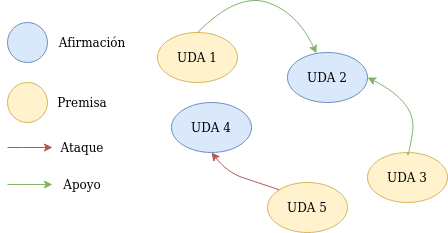
\includegraphics[scale=.7]{Graphics/Estructuras_argumentativas.png}
            % \includesvg[options]{Graphics/Estructuras argumentativas.svg}
        \end{center}
	    \caption{Estructuras Argumentativas}
	\end{center}
\end{figure}\label{fig:arg_struct}

\chapter{Marco teórico}\label{chapter:background}

En este capítulo se introducen conceptos de Aprendizaje Automático (AA). Temas
como la representación de datos, arquitecturas y evaluación de modelos son tratados en sus secciones.
Luego, se hace un recorrido por las diferentes investigaciones recientes realizadas en la EA, viendo
los enfoques desarrollados y la evolución de estos a partir del desarrollo e introducción de nuevos métodos en el
campo. Por último, se introduce la proyección de corpus, técnica necesaria para la creación de conjuntos 
de datos para el entrenamiento de modelos de AA.

\section{Aprendizaje Automático}

Existen varios problemas para los cuales es difícil escribir un programa de forma tradicional que pueda
resolverlo, como decir si en una imagen existe un gato o un perro, o transcribir una grabación. En el caso
de que se escribiera este programa probablemente sería frágil y poco escalable. El AA constituye el 
estudio de técnicas que pueden aprender de la experiencia [\cite{d2l}] y mediante su uso 
se puede automatizar el proceso de encontrar soluciones a dichos problemas, haciendo que sus resultados sean 
robustos y escalables. 

En AA existen tres tipos de aprendizaje:
\begin{itemize}
	\item Aprendizaje no supervisado: trabaja con datos no anotados y los algoritmos tratan de 
	extraer información de estos.
	\item Aprendizaje reforzado: trabaja en la creación de agentes que interactúen con 
	un ambiente obteniendo información de qué tan buenas son las acciones realizadas.
	\item Aprendizaje supervisado: trabaja con datos anotados y los algoritmos tratan de minimizar
	el error cometido en las predicciones.
\end{itemize}
A este útlimo principalmente se refiere esta sección.

Los componentes básicos de un problema de aprendizaje supervisado se pueden resumir en los datos de los que 
aprender, el modelo para transformar los datos, una función de pérdida que cuantifica qué tan malo o bueno es el 
modelo y un algoritmo que ajuste los parámetros del modelo para minimizar la pérdida.

Matemáticamente, un modelo constituye una función $\hat{y} = f_{\theta}(x)$ cuyo argumento son las 
representaciones de las entradas orginales $x$ y devuelve una salida $\hat{y}$. Esta función $f$ se encuentra
parametrizada por el vector $\theta$ el cual constituye los parámetros en los que el modelo se basa para realizar sus
cálculos. La función de pérdida se puede definir como $e(y, \hat{y})$, donde $y$ es el resultado esperado para $x$. 
El objetivo final del algoritmo de ajuste es encontrar $\theta$ tal que:

\begin{equation}
	\arg \min_{\theta} e(y, f_{\theta}(x))
\end{equation}\label{eq:arg_min_theta}.

Los parámetros $\theta$ eventualmente se van ajustando con algún algoritmo de optimización para que 
la función de error alcance un valor óptimo, aunque un óptimo global en la práctica es difícil de conseguir
debido a la complejidad del espacio de búsqueda.

Una manera de observar la complejidad de estos modelos sería la cantidad de capas de procesamiento que lo integran.
Los primeros modelos empezaron utilizando una sola capa\footnote{A estos modelos se les conoce 
como \emph{shallow} o poco profundos.} para realizar 
las tareas, más tarde estos modelos fueron ganando en complejidad al superponerle otras, dando paso al 
aprendizaje profundo (\emph{Deep Learning}). La superposición se refiere
a la composición de funciones $f_i$ y $f_{i+1}$ de tal forma que la imagen de $f_i$ sea compatible con el dominio de 
$f_{i+1}$, entonces se obtiene $f_{i+2}(x) = f_{i+1}(f_i(x))$, al aplicar este esquema se pueden agregar múltiples
capas y profundizar $f$ tanto como se desee.


\subsection{Representación de datos}

La representación de los datos constituye una parte importante al modelar un problema. Esta 
es la encargada de presentar datos abstractos, como imágenes, párrafos o sonidos, en formas tratables
por los algoritmos. Generalmente, se buscan configuraciones que recojan la mayor cantidad de información 
de la entrada relevante al problema.

En el PLN los datos suele estar representados con distintos niveles de granularidad.
De menor granularidad a mayor se pueden ir mencionando los documentos, párrafos, oraciones, palabras y
caracteres. Estos elementos es posible representarlos mediante vectores que codifiquen propiedades
objetivas del problema a tratar como características morfológicas o semánticas de estos. Por ejemplo, 
los textos tienen una popular manera de representarse mediante vectores de TF-IDF [\cite{manning2008introduction}],
una desventaja de esta representación es que no toma en cuenta el orden de las palabras, por lo que 
la representación de \emph{no me gusta,} y \emph{no, me gusta} serían iguales aunque semánticamente 
sean opuestas. Para agregarle la información de orden a la representación se introducen los llamados 
$n-$gramas, los cuales toman en cuenta una ventana de tamaño $n$ para conformar conjuntamente una representación.
Este enfoque conlleva a la limitante de que solo un contexto finito está disponible para hacer las inferencias,
para esto finalmente se crean representaciones individuales para cada palabra, las cuales codifican 
información y la secuencia completa es introducida al modelo para realizar la inferencia.
La manera más simple de representar una palabra es mediante la representación \emph{one-hot}, 
en esta, a cada palabra se le asigna un índice y el vector resultante posee la dimensión del 
vocabulario y es rellenado con ceros en todos sus elementos excepto en el índice de la palabra, donde se le asigna 1.
Esta representación asume que las palabras son independientes entre sí y 
computacionalmente ocupan un espacio considerable. Existen otras representaciones 
que brindan información al algoritmo sobre la morfológia y la semántica de la palabra que representa.

Las características morfológicas son aquellas que describen cómo está formado el elemento a analizar.
Estas pueden ser extraídas con relativa facilidad, entre tales características se encuentran tamaño, 
cantidad, posición de palabras o párrafos, presencia de sufijos, prefijos, acentos u otros marcadores
en el texto. Las características semánticas presentan una mayor dificultad a la hora de ser extraídas.
Para esto se utilizan diferentes modelos que codifican esta información en vectores continuos conocidos como 
\emph{embeddings}, entre los modelos existentes se encuentran
word2vec [\cite{mikolov2013efficient}], 
\emph{Global Vectors} (GloVe) [\cite{pennington2014glove}], 
\emph{Bidirectional Encoder Representations from Transformers} (BERT) [\cite{devlin2018bert}],
entre otros.

\subsection{Modelación de problemas}

Los problemas en la vida real se presentan en un principio como una descripción a un nivel de abstracción 
más alto que el requerido por los algoritmos existentes, se hablan de entidades abstractas como imágenes,
sonidos, textos o usuarios, además de la información que se desea extraer o las operaciones que se
desean aplicar sobre estas entidades. A lo largo del desarrollo del AA han aparecido diferentes tipos de problemas 
que aparecen frecuentemente en la práctica y sus respectivas maneras de solucionarlos. Uno de estos tipos de problemas
es el de secuencia a secuencia (\emph{seq2seq}), cuyo objetivo es la conversión de una secuencia en un dominio de entrada a otra 
secuencia en un dominio de salida. Con este tipo de problemas se modelan tareas como traducción automática, en 
donde el dominio de entrada es texto en un lenguaje de partida y el dominio de salida es texto en un lenguaje de llegada.
Otro problema que se resuelve con este tipo de problemas es la segmentación de texto, cuya entrada es una lista de \emph{tokens}
y la salida son etiquetas que indican cuándo empieza y termina un segmento de texto. Las etiquetas utilizadas para 
la segmentación, generalmente, son:

\begin{itemize}
	\item B (\emph{begin}): representa el inicio del segmento.
	\item I (\emph{inside}): representa la continuación del segmento previamente iniciado.
	\item O (\emph{outside}): representa la no pertenencia a un segmento.
\end{itemize}

Este esquema presenta una versión más elaborada en la que se agregan dos clases que representan el final 
de un segmento E (\emph{end}) y un segmento de un solo elemento S (\emph{single}). La tarea anterior es 
utilizada como base para otra un poco más compleja, en la que, además de segmentar el texto, se desea 
clasificarlo. Para este problema se añaden meta etiquetas correspondientes a los tipos a identificar $C$ 
% TODO Anotación {no dices quien es O} se dice arriba: representa la no pertenencia a un segmento.
obteniendo un conjunto final $R = \{ B, I, E, S \} \times C \cup \{ O \}$. En tareas como la extracción de entidades
nombradas este método es empleado, donde el conjunto $C$ contiene las posibles categorías de entidades a identificar.

\subsection{Arquitecturas}

En aprendizaje profundo existen una gran cantidad de arquitecturas que se pueden utilizar para formar el modelo 
final. Estas deben de ser seleccionadas en dependencia de los datos y el problema a tratar, ya que sus diseños 
emulan diferentes operaciones sobre datos que pueden ser más beneficiosas en situaciones específicas.

\subsubsection{Capas densas}

El perceptrón consiste es una transformación lineal del vector de datos $\textbf{x}$ con un bias $b$ y 
luego aplicar una transformación no lineal $g$, conocida como función de activación, 
para la obtención del resultado final:

\begin{equation}
	f(\textbf{x}) = g(\textbf{w}\textbf{x} + b).
\end{equation}

El perceptrón constituye la unidad básica de las capas densas, ya que estas consisten en la aplicación
de este modelo varias veces sobre la misma entrada $\textbf{x}$ produciendo vectores de la dimensión $k$ 
deseada como salida final. Los parámetros se codifican en la matriz $\textbf{W}$ y sus bias en el vactor $b$:

\begin{equation}
	f(\textbf{x}) = g(\textbf{Wx} + \textbf{b}).
\end{equation}

Para las funciones de activación existen varias elecciones. Una de estas es la función sigmoidal. 
Esta devuelve un valor entre 0 y 1, es usada en tareas de regresión logística. 
Se puede interpretar como el nivel de activación de la neurona:

\begin{equation}
	sigm(x) = \frac{1}{1-e^{-x}}.
\end{equation}

\emph{Rectified Linear Unit} (ReLU) se define como la parte positiva del argumento. Una ventaja que trae esta 
función de activación es su rápido cálculo de su derivada y que previene en parte de los problemas 
de desaparición de gradiente de la sigmoidal:

\begin{equation}
	relu(x) = \max(0, x).
\end{equation}

La función de activación \emph{softmax} es diferente a las anteriores en el sentido que necesita
el vector salida de la capa anterior para ser computada. Esta función convierte las $q$ salidas
en una distribución de probabilidad, algo necesario en tareas de clasificación:

\begin{equation}
	softmax_k(\textbf{x}) = \frac{e^{x_k}}{\sum\limits_{i=1}^{q} e^{x_i}}.
\end{equation}

\subsubsection{Redes Neuronales Convolucionales}

Las redes neuronales convolucionales (CNN, en inglés) 
son un tipo de redes usadas
principalmente para tratar datos donde su estructura espacial es relevante, por ejemplo,
en datos bidimensionales como imágenes y en unidimensionales como sonido y texto.
Estas redes aplican de una función de kernel sobre los datos, $f * g$ donde $f$ son los
datos, $g$ es el kernel o filtro y $*$ es el operador de convolución [\cite{d2l}]. La función $g$ se puede 
aprender en el proceso o también puede ser una función de agrupación predefinida. 
Un ejemplo bidimensional de una función de kernel se muestra en la Figura \ref{fig:conv_kernel}.

\begin{figure}[h!]
	\begin{center}
		\begin{center}
			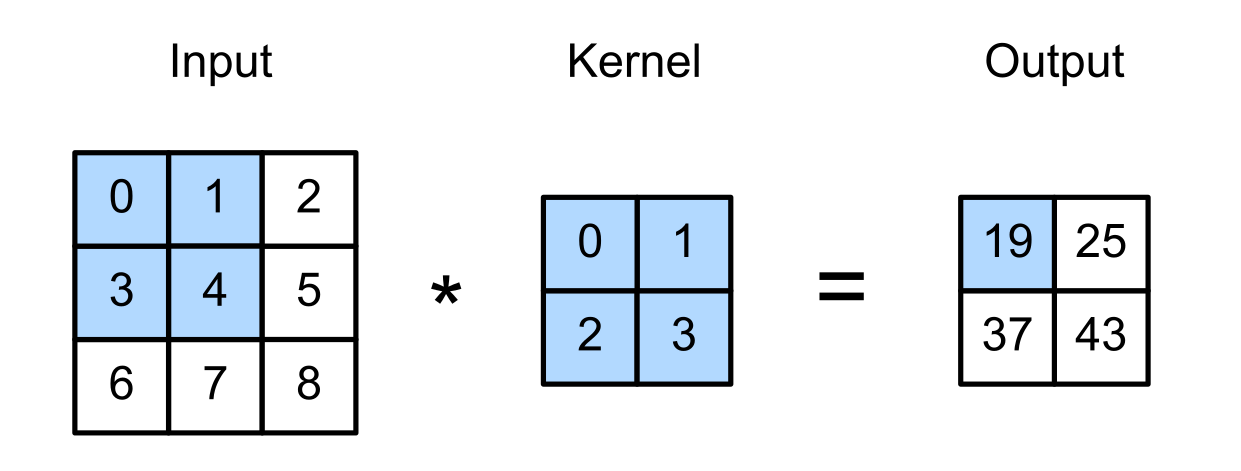
\includegraphics[scale=.2]{Graphics/kernel_convolution.png}
        \end{center}
		% TODO Cite problem, citar como texto
		% [\autocite{d2l}] 
		% [\parencite{d2l}] 
		% [\citet{d2l}] 
		% [\citep{d2l}] 
	    \caption{Convolución con kernel (Tomado de \cite{d2l} pág. 241).}\label{fig:conv_kernel}
	\end{center}
\end{figure}

En este se observa cómo una nueva representación es computada al operar el kernel por la matriz de datos. Este
corrimiento se puede realizar de diferentes formas, por ejemplo, se puede mover de dos en dos en vez de uno en uno, este
parámetro se le conoce como tamaño de paso (\emph{stride}). Es posible además preservar las dimensiones
iniciales de los datos al aplicarle un aumento de los datos en los bordes de tal forma que el resultado sea de la misma
dimensión, este aumento se realiza, generalmente, rellenando convenientemente los espacios con ceros, 
a esto se le llama \emph{padding} (Figura \ref{fig:conv_kernel_padding}).

\begin{figure}[h!]
	\begin{center}
		\begin{center}
			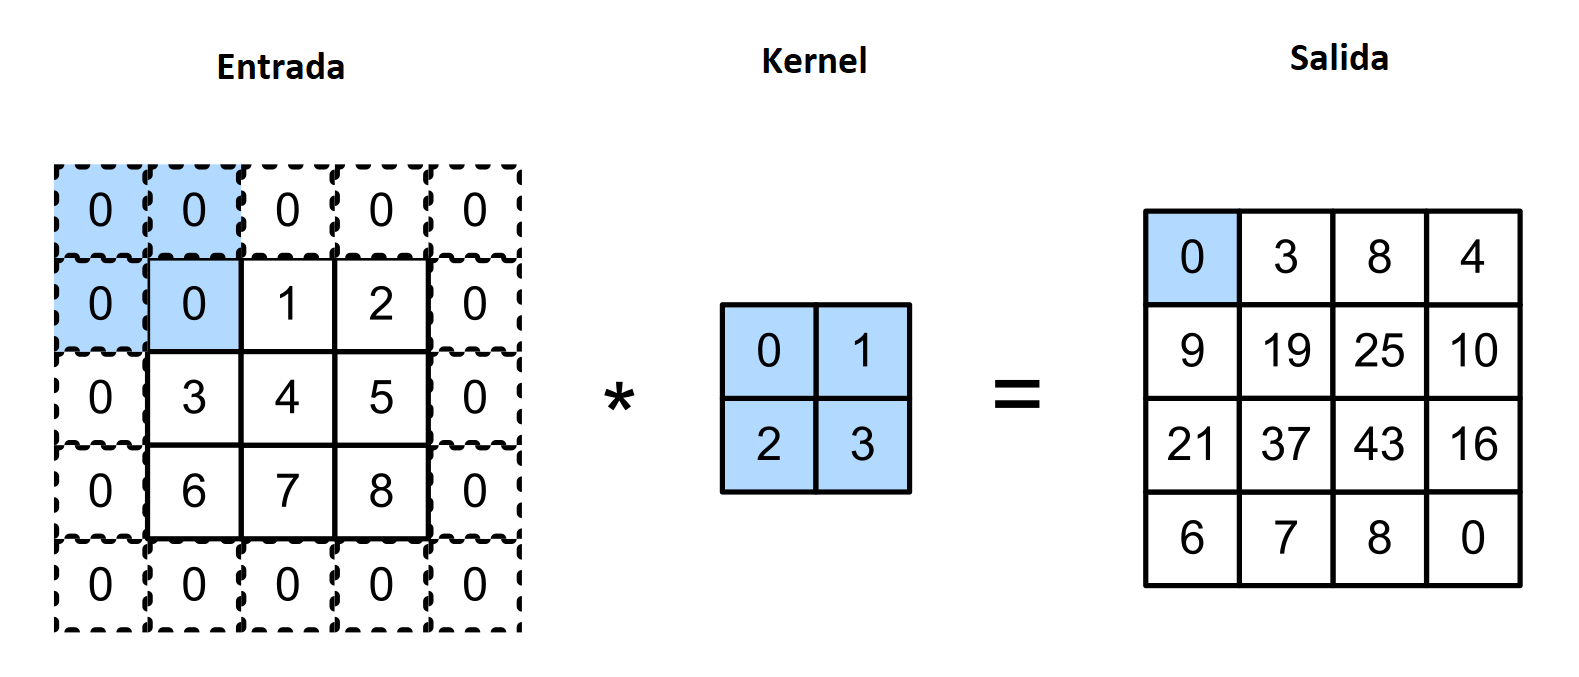
\includegraphics[scale=.2]{Graphics/kernel_convolution_padding.png}
        \end{center}
		% TODO Cite problem, citar como texto
		% [\autocite{d2l}] 
		% [\parencite{d2l}] 
		% [\citet{d2l}] 
		% [\citep{d2l}] 
		\caption{Convolución con kernel con \emph{padding} (Tomado de \cite{d2l} pág. 241).}\label{fig:conv_kernel_padding}
	\end{center}
\end{figure}

Existen varias funciones de agrupación usadas. Entre estas se encuentran las de agrupación máxima y de 
agrupación media. Como sus nombres indican, la de agrupación máxima devuelve el valor máximo de los encontrados
en la ventana del kernel, la de media calcula el promedio de estos valores. Estas capas tienen la capacidad de obtener
información resumida sobre los datos.

\subsubsection{Redes Residuales}

Al crear modelos de aprendizaje profundo se tienen un conjunto de parámetros $\theta$. Las posibles combinaciones 
de estos forman un espacio de funciones $F$ al cual pertenencen todas las posibles instancias del modelo.
Agregar nuevas capas aumenta la complejidad de este, pero no hay garantía de que el viejo espacio 
de funciones $F$ sea subconjunto del nuevo espacio $F'$, lo que implica que el nuevo modelo no es necesariamente
estrictamente superior al antiguo. Este problema es la razón para la aparición de las Redes Residuales. 
Una red residual está formada por 
uno o varios bloques residuales, en los que a la salida de cada bloque residual le es sumada la entrada de 
este mediante una conexión residual.
El objetivo de realizar tal operación es que es posible hacer la contribución del bloque 0 obteniendo así
un modelo equivalente a uno sin el bloque, garantizando la condición de subconjunto $F \subset F'$, además,
dicho bloque no pierde poder expresivo dado que en caso de que su aporte al resultado final sea considerable, 
se tendría que aprender solamente la función $f(x) - x$ donde $x$ es la entrada del bloque y $f$ es la función 
aprendida por el bloque sin la conexión residual, para mitigar el efecto de la conexión residual como se muestra
en la Figura \ref{fig:res_block}.

\begin{figure}[h!]
	\begin{center}
		\begin{center}
			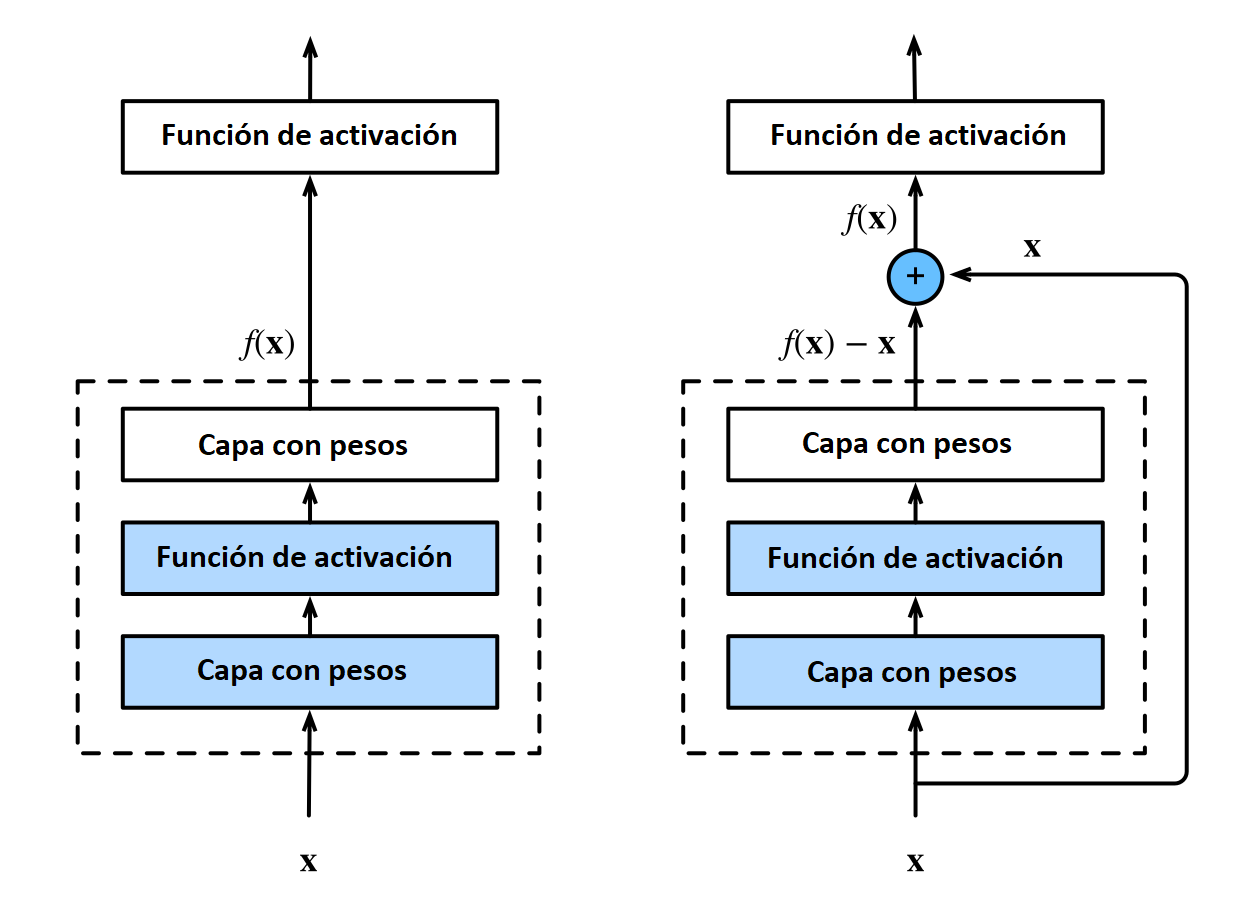
\includegraphics[scale=.3]{Graphics/resnet.png}
        \end{center}
		% TODO Cite problem, citar como texto
		% [\autocite{d2l}] 
		% [\parencite{d2l}] 
		% [\citet{d2l}] 
		% [\citep{d2l}] 
	    \caption{Bloque residual (Tomado de \cite{d2l} pág. 289).}\label{fig:res_block}
	\end{center}
\end{figure}

\subsubsection{Redes Neuronales Recurrentes}

Las redes neuronales recurrentes (RNN, en inglés) son
un tipo especial de arquitectura especializada en el trabajo con datos secuenciales. Este tipo de arquitectura
presenta variables en las que se almacenan información pasada, que es usada para el computo de la salida. El 
problema se puede modelar probabilísticamente mediante la estimación de $P(x_t | x_{t-1}, \dots, x_{1})$,
donde existen dos variantes principales. En una variante se fija un tamaño de ventana en el tiempo $\alpha$ 
dando como resultado $P(x_t | x_{t-1}, \dots, x_{t-\alpha})$, a este tipo de modelos se les conoce como autoregresivos. 
Otra estrategia consiste en guardar un contexto de observaciones pasadas $h_t$ y con este realizar la estimación 
$P(x_t | h_t)$, el contexto se actualiza en cada paso mediante una función $h_t = g(h_{t-1}, x_{t-1})$, a estos 
se les nombra modelos autorregresivos latentes, debido a la existencia de variables ocultas $h_t$. 

En la práctica estos modelos presentan problemas de gradientes, ya que estas pueden volverse extremadamente grandes o 
desaparecer.
Para esto se han creado arquitecturas que disminuyen estos problemas. Una de estas arquitecturas es las de memorias
de corto largo plazo (LSTM, en inglés) [\cite{hochreiter1997long}].
Este modelo guarda un contexto del procesamiento y está constituído por varias compuertas que regulan las 
actualizaciones de los estados internos. LSTM (Figura \ref{fig:rnn_lstm}) posee dos variables de estado, la memoria 
$C$ y el estado oculto $H$. Entre sus compuertas se encuentran la compuerta de olvido, esta regula cuánto de la 
memoria permanece en el próximo paso, la compuerta de entrada ajusta la cantidad de información nueva que entrará, 
la compuerta de salida maneja el cálculo del próximo estado oculto.

\begin{figure}[h!]
	\begin{center}
		\begin{center}
			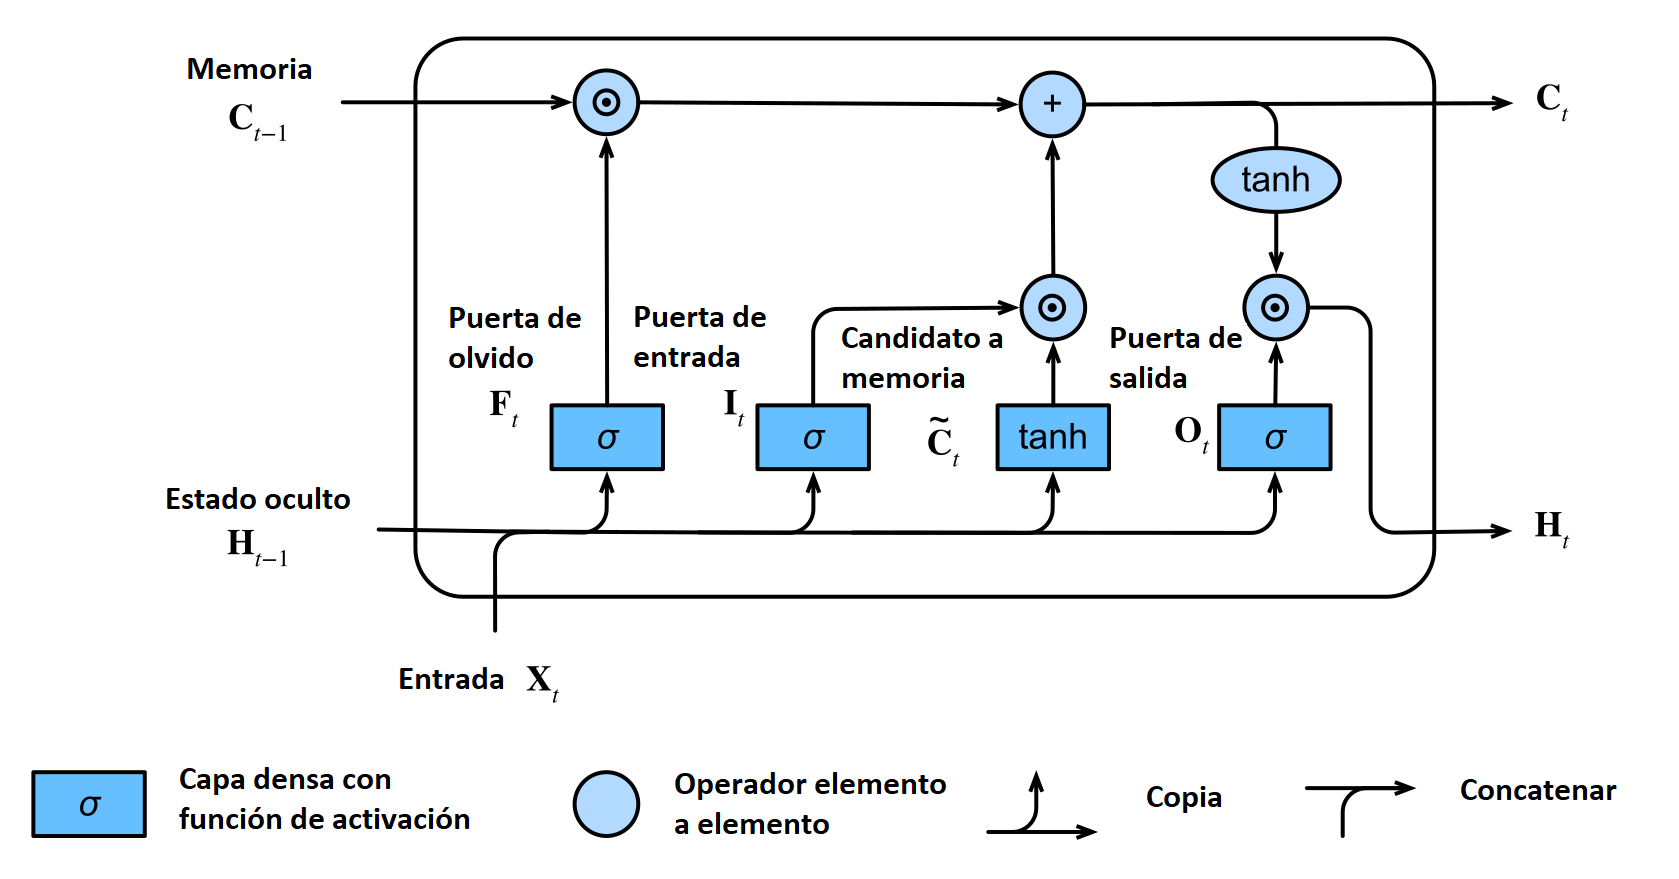
\includegraphics[scale=.3]{Graphics/rnn_lstm.png}
        \end{center}
		% TODO Cite problem, citar como texto
		% [\autocite{d2l}] 
		% [\parencite{d2l}] 
		% [\citet{d2l}] 
		% [\citep{d2l}] 
	    \caption{LSTM (Tomado de \cite{d2l} pág. 357).}\label{fig:rnn_lstm}
	\end{center}
\end{figure}

El método de aprendizaje de las RNN solamente observa los elementos anteriores de la secuencia, aunque existen
tareas en las que, observando los elementos posteriores, brinda más contexto e información a la tarea, sin que interfiera
en el proceso de inferencia. El modelo bidireccional presenta una alternativa para tratar con este tipo de problemas, 
este modelo consiste en, además de hacer el recorrido de inicio a final de la secuencia, realizar otro recorrido en orden 
inverso, estos recorridos van generando dos estados ocultos $\overrightarrow{H}_{i}$ y $\overleftarrow{H}_{i}$
que luego son mezclados para obtener el contexto final $H_i$, los tipos de mezclas comunes son la concatenación de los 
estados o la multiplicación elemento a elemento de estos.

\begin{figure}[h!]
	\begin{center}
		\begin{center}
			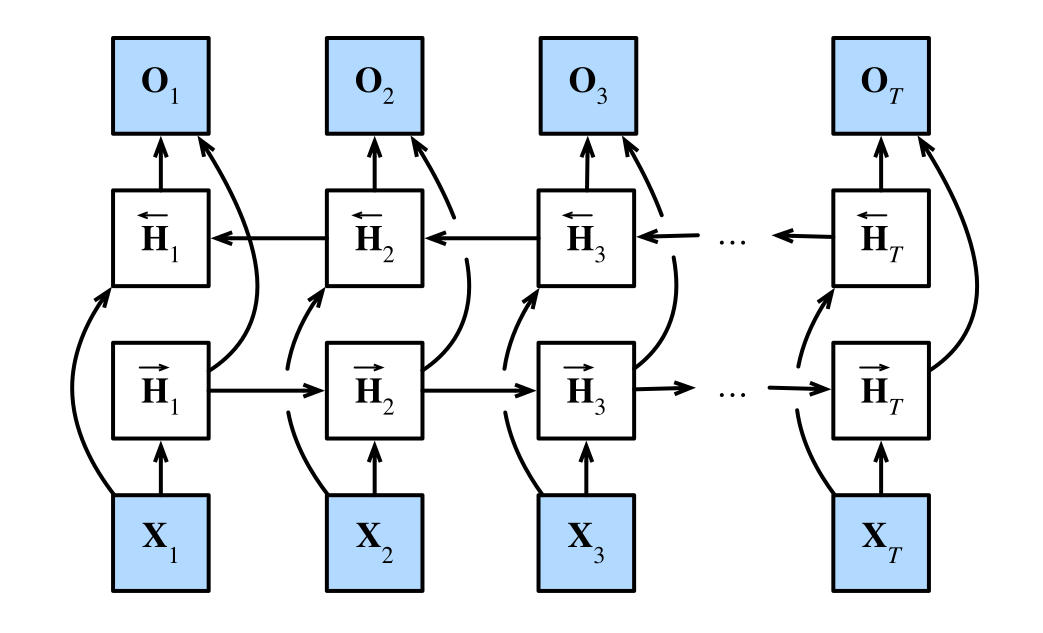
\includegraphics[scale=.3]{Graphics/rnn_bidirectional.png}
        \end{center}
		% TODO Cite problem, citar como texto
		% [\autocite{d2l}] 
		% [\parencite{d2l}] 
		% [\citet{d2l}] 
		% [\citep{d2l}] 
	    \caption{Red neuronal bidireccional (Tomado de \cite{d2l} pág. 367).}\label{fig:rnn_bidirectional}
	\end{center}
\end{figure}


\subsubsection{Atención}

% Definicion, qué hace, uso en secuencias
La atención es una técnica en la cual se hace una selección ponderada de atributos en un contexto específico. 
Este mecanismo presenta dos partes, una consulta $q$ y una colección de pares llave-valor, $(k_i, v_i)$. La 
consulta representa el contexto en donde se quiere aplicar la atención y las llaves $k_i$ son elementos que 
relacionan la consulta a los valores $v_i$. El proceso de calcular el resultado consiste en, primero, calcular 
el vector compatibilidad $e$ entre las llaves y la consulta mediante la función $f$, este vector es luego 
modificado por una función $g$ que distribuye los valores obteniendo el vector atención $a$. Finalmente 
este vector es utilizado para calcular el resultado final al aplicarle la función $o = z(a, V)$:

\begin{equation}
	e = f(q, K),
\end{equation}
\begin{equation}
	a = g(e),
\end{equation}
\begin{equation}
	o = z(a, V).
\end{equation}

En dependencia de cómo se seleccionen las funciones $f$, $g$ y $z$ se pueden obtener distintos tipos de atención.
Una configuración simple consiste en definir $f$ como el producto punto de la consulta con la llave,
$g$ como \emph{softmax} y $z$ la suma ponderada de $v_i$ con los valores de atención.

\subsubsection{Campo Aleatorio Condicional}

% Definicion de CRF, qué modela, Ventajas de CRF en secuencias, mirar relacion con Hidden Markov Models

El campo aleatorio condicional (CRF, en inglés) es un 
tipo de modelo gráfico probabilístico que modela eficientemente el trabajo con secuencias
% TODO PREGUNTAR {modelando} se cambia para s y luego de {conjuntamente} se se pone con? 
modelando conjuntamente la probabilidad de las etiquetas de las secuencias, dadas sus observaciones [\cite{lafferty2001conditional}].
En trabajos de secuencias, la forma más simple que toma el grafo consiste en una cadena de las variables representando
las etiquetas de las secuencias $Y$, conectadas de la forma $(Y_i, Y_{i+1})$ y las variables observadas $X$, conectadas
a las variables $Y$ [\cite{wallach2004conditional}].

El objetivo de CRF es calcular la secuencia $Y^*$ tal que:

\begin{equation}
	Y^* = \arg \max_Y P(Y | X).
\end{equation}\label{eq:crf}

En esta expresión se observa que devuelve la secuencia más probable, dadas las variables observadas o atributos $X$,
por lo que esta capa es usada al final del proceso para problemas de clasificación de secuencias.

\subsection{Evaluación del modelo y métricas}

Los modelos de AA necesitan maneras de expresar qué tan buenos son 
en las tareas encomendadas. Para esto se crean funciones que evalúan los resultados obtenidos
por dichos modelos, estas funciones se les da el nombre de métricas. Existen diferentes tipos de
métricas para tratar con diferentes tipos de problemas. En aprendizaje supervisado una métrica se
define como una función $m_s(Y, \hat{Y})$, donde $Y$ son las predicciones verdaderas y $\hat{Y}$ son las predicciones
hechas por el modelo. En algoritmos de aprendizaje no supervisado como K-Means y K-NN son usadas funciones $m_{ns}(\hat{Y})$
donde $\hat{Y}$ son las predicciones finales. En comparación con su versión supervisada estas funciones no tiene acceso
a las predicciones verdaderas del problema.

\subsubsection{Clasificación}

En problemas de clasificación (problemas en donde las etiquetas a predecir son discretas) 
son empleadas medidas que toman en cuenta la naturaleza discreta de su conjunto imagen.
Medidas como precisión, recobrado, \emph{accuracy} y F1 son utilizadas en la 
evaluación de los resultados, mientras que como función de error se usa entropía cruzada 
(\emph{cross entropy} en inglés) [\cite{grandini2020metrics}].

La matriz de confusión es una vía de representar los resultados de dos clasificadores. Esta matriz en $M_{ij}$ 
indica la cantidad de elementos que clasificó como clase $i$ el primer clasificador y
como clase $j$ el segundo clasificador. En su uso práctico,
un clasificador son las etiquetas verdaderas mientras que el otro es el clasificador que se está evaluando. 
En problemas de la clasificación binaria, donde se busca saber si existe pertenencia o no de un elemento a una clase,
se pueden observar los siguientes casos:

\begin{itemize}
	\item Verdaderos Positivos (VP): elementos clasificados correctamente que pertenecen a la clase.
	\item Verdaderos Negativos (VN): elementos clasificados correctamente que no pertenecen a la clase.
	\item Falsos Positivos (FP): elementos clasificados incorrectamente que pertenecen a la clase.
	\item Falsos Negativos (FN): elementos clasificados incorrectamente que no pertenecen a la clase.
\end{itemize}

\begin{table}[h!]
	\begin{center}
		\begin{tabular}{|c|c|c|} \hline
		Clases		& Positivo	& Negativo  \\ \hline
		Positivo	& VP  		& FN		\\ \hline
		Negativo	& FP		& VN		\\ \hline
		\end{tabular}
	\caption{Matriz de confusión binaria.}\label{fig:confusion_matrix}
	\end{center}
\end{table}

La precisión es la medida que indica la probabilidad de que la clasificación de una clase sea correcta. Esto 
se puede observar como la proporción de los elementos correctamente clasificados sobre el total de 
elementos clasificados:

\begin{equation}
	prec_i = \frac{VP}{VP + FP}.
\end{equation}

En problemas de clasificación múltiple surge la versión macro de esta medida calculada como la media de todas
las precisiones de las clases existentes:

\begin{equation}
	prec_{macro} = \sum^K_{i=1} \frac{prec_i}{K}.
\end{equation}

El recobrado es la medida que indica la probabilidad de que se clasifique correctamente un elemento de la clase
del total existente. Esto se puede observar como la proporción de los elementos correctamente clasificados sobre el 
total de elementos que pertenecen a la clase:

\begin{equation}
	rec_i = \frac{VP}{VP + FN}.
\end{equation}

En problemas de clasificación múltiple surge la versión macro de esta medida calculada como la media de todos
los recobrados de las clases existentes:

\begin{equation}
	rec_{macro} = \sum^K_{i=1} \frac{rec_i}{K}.
\end{equation}

La medida F1 es la media armónica de la precisión y el recobrado. En esta la contribución de la precisión y el
recobrado al resultado final es el mismo, aunque es posible buscar variaciones de acuerdo a al problema a tratar:

\begin{equation}
	F1_i = 2 \frac{prec_i \cdot rec_i}{prec_i + rec_i}.
\end{equation}

En problemas de clasificación múltiple surge la versión macro de esta medida calculada la propia medida F1, pero
utilizando la precisión y recobrado macro del problema:

\begin{equation}
	F1_{macro} = 2 \frac{prec_{macro} \cdot rec_{macro}}{prec_{macro} + rec_{macro}}.
\end{equation}

La métrica $alpha$\%F1 [\cite{persing2016end}] es una métrica basada en la idea de F1 orientada para el 
trabajo con secuencias donde $\alpha$ denota el porcentaje de secuencia inferida que debe coincidir con 
la secuencia anotada para ser considerado una coincidencia. Esta versión permite
establecer el rango de flexibilidad si $\alpha=100$ (100\%F1), significa que deben coincidir completamente, 
mientras si $\alpha = 50$ (50\%F1) significa que, si coinciden en una proporción mayor o igual a la mitad, 
se considera como un verdadero positivo. La definición de los valores de verdaderos positivos, negativos 
y falsos negativos es:

\begin{equation}
	VP = |\{ j | \exists i | gl(j) = pl(i) \land i = j \}|,
\end{equation}
\begin{equation}
	FP = |\{ i | pl(i) \neq n \land \not\exists j | gl(j) = pl(i) \land i = j \}|,
\end{equation}
\begin{equation}
	FN = |\{ j | \not\exists i | gl(j) = pl(i) \land i = j \}|,
\end{equation}

donde $i$ y $j$ son las UDAs extraídas, $gl(j)$ es la etiqueta correcta para $j$, $pl(i)$ es 
la etiqueta inferida para $i$, $n$ es la clase no argumentativa, $i = j$ significa que $i$ es 
una coincidencia para $j$.

Las métricas anteriores están acotadas por los valores 0 y 1, donde 1 representa la mejor evaluación y 0 la 
peor.

La entropía cruzada se encarga de evaluar qué tan diferentes son dos funciones de distribución $p$ y $q$, su 
resultado es un número no negativo que, a medida que sean más pequeños los valores, indican mayor similitud. 
En su versión discreta se formula así:

\begin{equation}
	H(p, q) = - \sum_{x \in D} p(x) \log q(x).
\end{equation}

\subsubsection{Cadenas}

Para textos o cadenas existen diferentes métricas que constituyen formas de saber la similitud 
entre dos elementos. Una de esas métricas es la similitud de Jaccard, esa se puede ver como una 
la proporción de elementos comunes que presentan dos conjuntos, los elementos sería palabras:

\begin{equation}
	jac(X, Y) = \frac{|X \cap Y|}{|X \cup Y|}.
\end{equation}.
Otra medida de similitud es la distancia de Levenshtein, la cual se define como la mínima cantidad 
de cambios de eliminar, cambiar y agregar que se tienen que hacer a dos secuencias para que sean 
iguales. Esta medida se puede usar tanto en palabras, en donde se mediría la cantidad de cambios 
a los caracteres, como en listas de palabras, donde se mediría la cantidad de palabras que 
se tienen que cambiar. 

\subsubsection{Curvas de aprendizaje}

Es necesario además de evaluar el resultado final del modelo, evaluar el proceso de entrenamiento. En esta etapa 
se pueden diagnosticar varias deficiencias en este proceso. Para un correcto diagnóstico se divide el conjunto de 
datos en tres partes:

\begin{itemize}
	\item \textbf{entrenamiento}: utilizada para el entrenamiento del modelo.
	\item \textbf{validación}: utilizada para evaluar el desempeño del modelo en entrenamiento.
	\item \textbf{prueba}: utilizada para evaluar el resultado final.
\end{itemize}

Las curvas de aprendizaje constituyen la principal herramienta para evaluar el proceso de aprendizaje.
Estas están formadas por las mediciones de métricas a lo largo del entrenamiento calculadas a partir de 
los conjuntos de validación y entrenamiento. El eje horizontal representa el número de época del entrenamiento,
iteración sobre el conjunto de entrenamiento, y el eje vertical representa la métrica a analizar. 
La línea correspondiente al conjunto de entrenamiento cuantifica 
el aprendizaje del modelo o también el error de entrenamiento, y la correspondiente a la de validación cuantifica 
la generalización o el error de generalización. Existen tres comportamientos escenciales:

\begin{itemize}
	\item Bajo ajuste (\emph{underfitting}).
	\item Sobreajuste (\emph{overfitting}).
	\item Buen ajuste.
\end{itemize}

El bajo ajuste ocurre cuando el modelo no es capaz de aprender del conjunto de datos o cuando este aún puede aprender 
más. Las curvas de aprendizaje en estos casos se caracterizan por ser una linea plana o valores ruidosos con alta pérdida
(Figura \ref{fig:underfit}).

\begin{figure}[h!]
	\begin{center}
		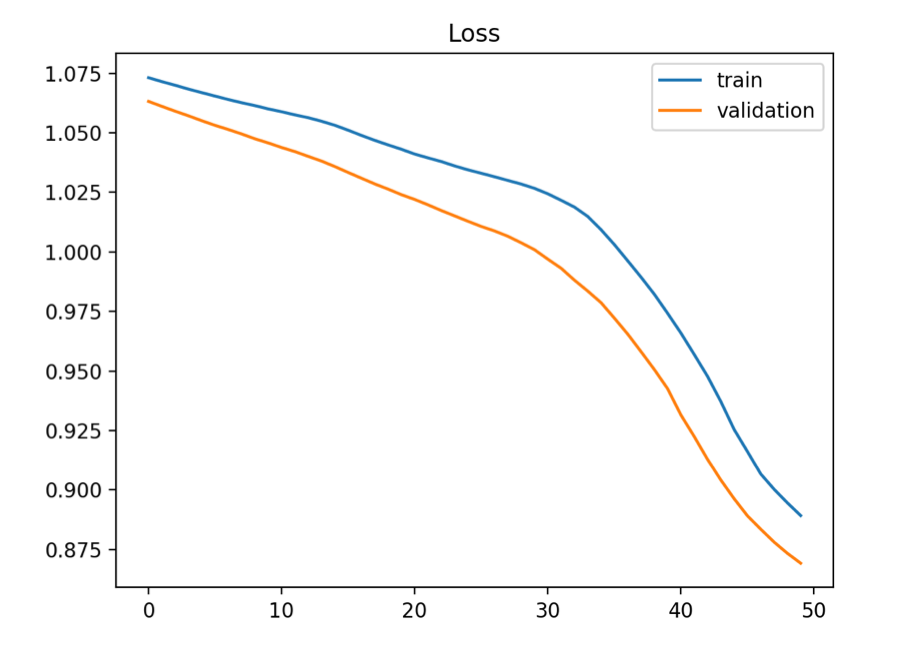
\includegraphics[scale=.2]{Graphics/underfit_missing_training.png}
		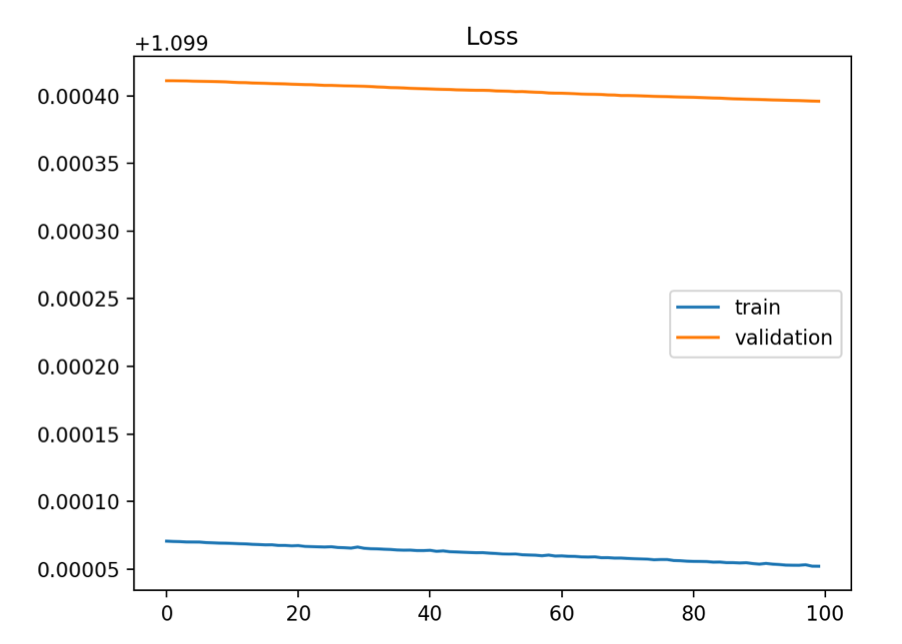
\includegraphics[scale=.2]{Graphics/underfit_not_learning.png}
		% TODO Cite problem, citar como texto
		% TODO PREGUNTAR, la página es en romano, luego de esas vienen páginas en números normales,
		% poner el número normal traería confusión
		% [\autocite{brownlee2018better}] 
		% [\parencite{brownlee2018better}] 
		% [\citet{brownlee2018better}] 
		% [\citep{brownlee2018better}] 
		\caption{Curvas de entrenamiento con bajo ajuste por falta de entrenamiento (izquierda) 
		y por modelo que no aprende de los datos (derecha) (Tomado de \cite{brownlee2018better} pág. XXVII).}\label{fig:underfit}
	\end{center}
\end{figure}

Entre las formas más sencillas de combatir el bajo ajuste de los modelos consiste en complejizar el modelo, al añadir
capas o aumentar las dimensiones de este aumenta su expresividad y, por lo tanto, su ajuste. Si este método 
no funciona es posible considerar un cambio de arquitectura hacia una que pueda extraer más información de la 
estructura de los datos. 

El sobreajuste es el fenómeno en el que el modelo aprende los datos de entrenamiento extremadamente bien, incluso
el ruido en estos, esto trae consigo que falla en generalizar el problema para nuevas entradas. Las curvas 
características de este fenómeno presentan una divergencia en los errores de entrenamiento y validación a medida
que se entrena el modelo, mientras que la de entrenamiento mejora la de validación tiende a empeorar (Figura \ref{fig:overfit}). 

\begin{figure}[h!]
	\begin{center}
		\begin{center}
			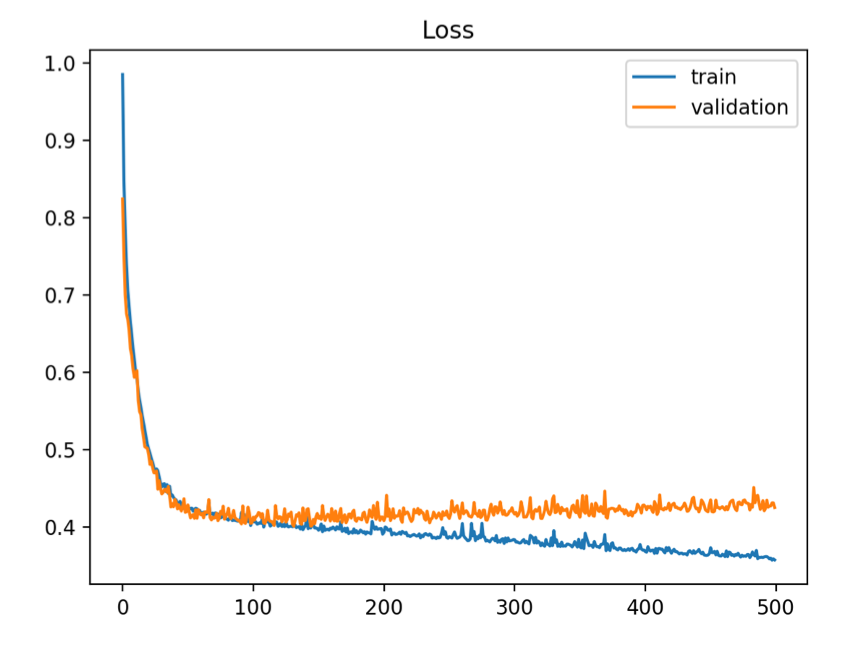
\includegraphics[scale=.3]{Graphics/overfit_raising_val_error.png}
        \end{center}
		% TODO Cite problem, citar como texto
		% TODO PREGUNTAR, la página es en romano, luego de esas vienen páginas en números normales,
		% poner el número normal traería confusión
		% [\autocite{brownlee2018better}] 
		% [\parencite{brownlee2018better}] 
		% [\citet{brownlee2018better}] 
		% [\citep{brownlee2018better}] 
	    \caption{Curvas de entrenamiento con sobreajuste (Tomado de \cite{brownlee2018better} pág. XXIX).}\label{fig:overfit}
	\end{center}
\end{figure}

Existen varios métodos para combatir el sobreajuste, uno sencillo es simplificar el modelo quitándole capas 
o disminuyendo sus dimensiones. Además de esto, existen regularizaciones que se pueden aplicar para evitar que 
las capas dependan exclusivamente de pocos atributos, entre esta familia los más usados son la regularización
L1 y L2 las cuales se definen como la suma del valor absoluto de los atributos y la suma del cuadrado de sus 
atributos respectivamente. Otra medida para prevenir el sobreajuste es el agrego de capas de abandono 
(\emph{dropout}). Estas capas desactivan neuronas de la arquitectura y obligando a 
estas a ser robustas y depender del comportamiento de la población, en lugar de la actividad de otras unidades 
específicas [\cite{baldi2013dropout}]. La terminación temprana (\emph{early stopping}) del entrenamiento
se utiliza para parar este en el momento en que el error de generalización comienza a subir, impidiendo así que 
se sobreentrene el modelo.

Finalmente, un buen ajuste es el resultado que se alcanza cuando tanto la curva de validación como de entrenamiento
presentan valores pequeños y similares, consecuentes con una correcto aprendizaje y generalización (Figura \ref{fig:good_fit}).

\begin{figure}[h!]
	\begin{center}
		\begin{center}
			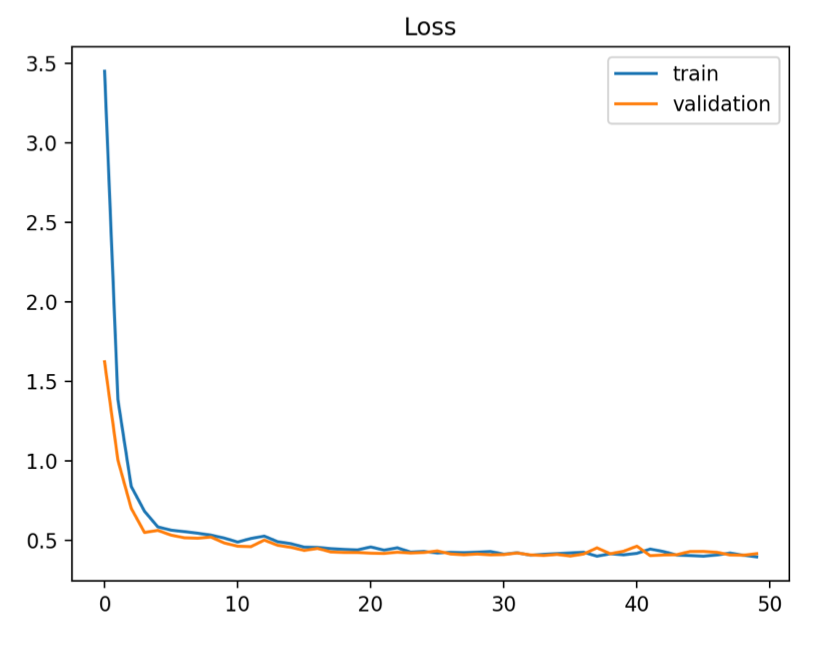
\includegraphics[scale=.3]{Graphics/good_fit.png}
        \end{center}
		% TODO Cite problem, citar como texto
		% TODO PREGUNTAR, la página es en romano, luego de esas vienen páginas en números normales,
		% poner el número normal traería confusión
		% [\autocite{brownlee2018better}] 
		% [\parencite{brownlee2018better}] 
		% [\citet{brownlee2018better}] 
		% [\citep{brownlee2018better}] 
	    \caption{Curvas de entrenamiento con buen ajuste (Tomado de \cite{brownlee2018better} pág. XXX).}\label{fig:good_fit}
	\end{center}
\end{figure}

Otro problema observable a partir del análisis de las curvas de aprendizaje constituye la detección de conjuntos
de datos no representativos. Un conjunto de datos no representativo es uno que puede no 
capturar las características estadísticas relativas a otro conjunto de datos extraído del mismo dominio.
Esto puede pasar que los conjuntos de entrenamiento o de validación. En caso del conjunto de entrenamiento
se puede identificar si la pérdida en el conjunto de entrnamiento conlleva a una ganancia en el conjunto de 
validación y viceversa quedando al final con una separación entre ambos valores. En el caso del conjunto de 
validación se presenta como una curva ruidosa, también se puede dar el caso de que el conjunto  de validación
sea más fácil de predecir que el de entrenamiento, en este caso se observa como la curva de validación permanece
siempre por debajo de la de entrenamiento (Figura \ref{fig:unrepresentative_data}).

\begin{figure}[h!]
	\begin{center}
		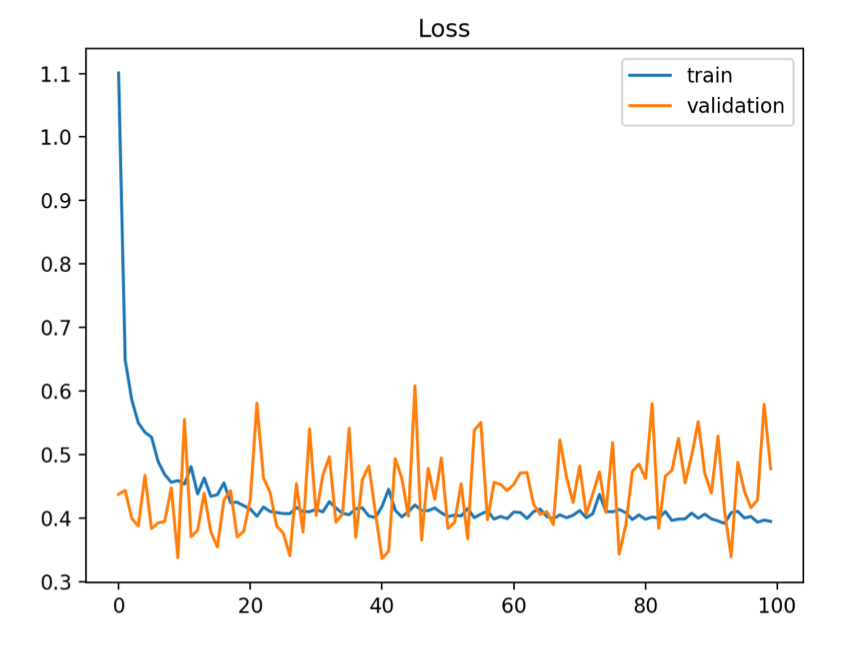
\includegraphics[scale=.2]{Graphics/unrepresentative_dev_set.png}
		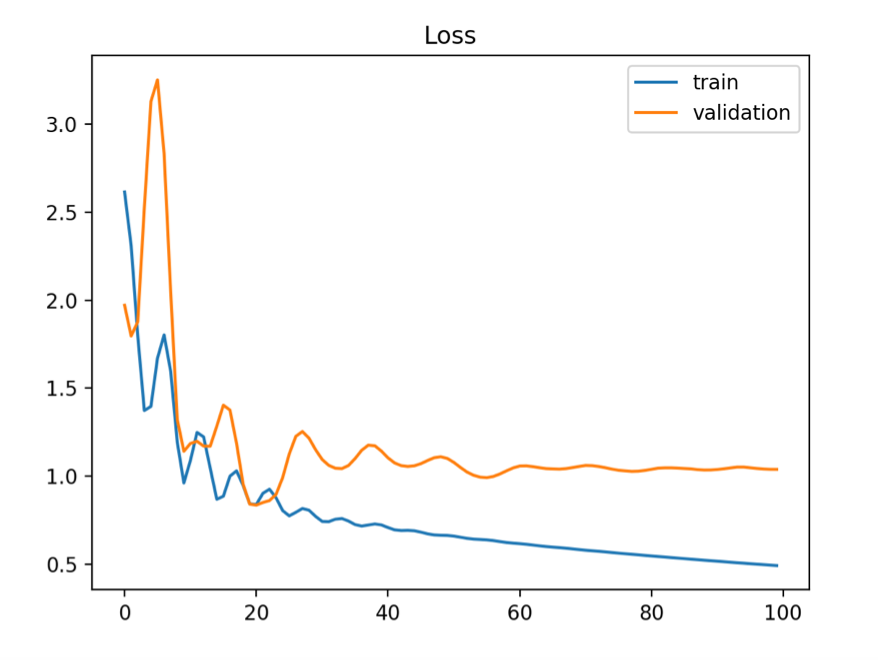
\includegraphics[scale=.2]{Graphics/unrepresentative_train_set.png}
		% TODO Cite problem, citar como texto
		% TODO PREGUNTAR, la página es en romano, luego de esas vienen páginas en números normales,
		% poner el número normal traería confusión
		% [\autocite{brownlee2018better}] 
		% [\parencite{brownlee2018better}] 
		% [\citet{brownlee2018better}] 
		% [\citep{brownlee2018better}] 
		\caption{Curvas de entrenamiento con datos poco representativos en el conjunto de validación (izquierda) 
		y en el conjunto de entrenamiento (derecha) (Tomado de \cite{brownlee2018better} pág. XXXII).}\label{fig:unrepresentative_data}
	\end{center}
\end{figure}

Para combatir estos problemas se puede aumentar la cantidad de elementos en los conjuntos de entrenamiento o 
validación en dependencia de donde ocurra.

\subsection{Aumento de datos}

El aumento de datos consiste en acciones para aumentar la diversidad de un conjunto de datos sin recolectar
nuevos datos explícitamente [\cite{feng2021data}]. En datos continuos, como imágenes o valores numéricos el 
aumento de datos puede ser realizado al añadirle perturbaciones a entradas existentes, en caso de las imágenes 
técnicas como el volteado (\emph{flipping}) o recortado (\emph{cropping}) son usadas. Los textos son un tipo 
de datos discreto y, por lo tanto, las técnicas anteriores no pueden ser aplicadas directamente. Para el PLN
se han estudiado diversas técnicas de aumento de datos, una de estas consiste en el cambio del árbol de 
dependencia de la oración mediante operaciones de intercambio y borrado de nodos [\cite{csahin2019data}], también se han utilizado 
el intercambio de palabras por sinónimos [\cite{dai2020analysis}] y la traducción de textos hacia un lenguaje y luego 
de vuelta al lenguaje origen (\emph{backtranslation}) [\cite{sennrich2015improving}]. 

\subsection{Aprendizaje Conjunto}

El aprendizaje conjunto (\emph{ensemble learning}) son técnicas encaminadas al aprovechamiento
de soluciones encontradas por diferentes modelos, combinándolas y mejorándolas para encontrar una mejor solución 
al problema. Estos métodos son efectivos en la reducción de la varianza y el sesgo de los resultados, obteniendo así
mejores resultados [\cite{dietterich2002ensemble}]. Una forma de este tipo de aprendizaje en problemas de 
clasificación constituye el voto conjunto, en donde los diferentes clasificadores votan sobre la clase a la que 
pertenece el elemento y, al final, se asigna la etiqueta que más votos obtuvo.

\subsection{Métodos de optimización}

El objetivo de el AA es encontrar los extremos de una función de costo, este proceso es una tarea 
desafiante ya que la gran mayoría de estas funciones no son convexas y, por lo tanto, no existe un algoritmo
que asegure la convergencia hacia un extremo global. Para resolver este problema exiten múltiples heurísticas,
la más usada es el descenso por gradiente. La idea básica consiste 
en el cálculo del vector gradiente de la función de error $e$ con respecto a los parámetros del modelo $x$ y, una vez se 
tiene dicho vector, se evalúa en la asignación actual de los parámetros $x_i$ y se realiza un corrimiento de este punto 
% TODO PREGUNTAR dice sustituir por {dirección} contra. No debe ser así no? 
en contra del gradiente para disminuir el error (Eq. \ref{eq:gradien_descent}).

\begin{equation}
	x_{i+1} = x_i - \alpha \nabla f(x_i)\label{eq:gradien_descent}
\end{equation}

En la ecuación \ref{eq:gradien_descent} anterior, $\alpha$ es la tasa de aprendizaje (\emph{learning rate}),
que cuantifica cuánto se toma del vector de gradiente para actualizar los parámetros, esto 
se puede ver como el aprendizaje del modelo.

Variantes eficientes de este algoritmo para el entrenamiento de modelos de AA han sido 
creadas, las variaciones se encuentran principalmente en la selección de $\alpha$ en cada paso y la 
selección de los conjuntos de datos con que se estimará el gradiente. Entre las técnicas utilizadas se 
encuentran Descenso por Gradiente Estocástico, variaciones de tasa de aprendizaje dinámica con 
sus diferentes variantes (exponencial, polinómica), RMSProp [\cite{tieleman2012rmsp}] 
y Adam [\cite{kingma2014adam}].

\section{Preliminares de Extracción de Argumentos}

Varias investigaciones han dado respuesta a los problemas asociados a EA, mostrando
una variedad en enfoques y métodos.

% TODO Cite problem, citar como texto
% [\autocite{palau2009argumentation}] 
% [\parencite{palau2009argumentation}] 
% [\citet{palau2009argumentation}] 
% [\citep{palau2009argumentation}] 
En \cite{palau2009argumentation} se propone
el uso de modelos estadísticos como \emph{Naive Bayes} (NB) y \emph{Support Vector Machine} (SVM) 
para la clasificación de 
oraciones en argumentativas o no y en su rol argumentativo en caso de que sea argumentativa, en este
caso se asume que las componentes argumentativas son oraciones completas. Para la predicción de relaciones
se usa un enfoque basado en reglas con la creación de una Gramática Libre de Contexto. Las representaciones
de las oraciones consisten en atributos creados a mano, dado el conocimiento experto sobre la argumentación
en el tema tratado, elementos como adverbios, verbos, signos de puntuación, palabras clave, estadísticas del texto
(tamaño de oración, distancia media de palabras) son usados para la extracción y clasificación de las UDA, además,
se usan también como base en la creación de las reglas de la gramática para la extracción de relaciones.

% TODO Cite problem, citar como texto
% [\autocite{goudas2015argument}] 
% [\parencite{goudas2015argument}] 
% [\citet{goudas2015argument}] 
% [\citep{goudas2015argument}] 
\cite{goudas2015argument} al igual que \cite{palau2009argumentation} clasifica a las oraciones como
argumentativas o no, mediante diferentes clasificadores como NB, \emph{Random Forest}, Regresión
Logística y SVM. Sin embargo, \cite{goudas2015argument} aumenta la grandularidad de la segmentación al permitir
la extracción de los segmentos que contienen la carga argumentativa de dentro de las oraciones previamente clasificadas
como tal, esto se realiza mediante la extracción de etiquetas BIO de las oraciones con el uso de un 
CRF. La predicción de las relaciones es modelado como un problema de clasificación
% TODO PREGUNTAR dice eliminar {en}, pero no le veo el sentido a eso.
usando SVM para clasificar pares de UDAs en relacionados o no. Atributos creados a mano 
son usados en la extracción de UDAs; entre estos están posición de la oración en el texto, cantidad de verbos, comas, adverbios,
palabras, entidades en la oración, también se emplean gaceteras que guardan entidades relacionadas con el dominio 
específico y palabras clave indicadoras de frases argumentativas. 

% TODO Cite problem, citar como texto
% [\autocite{stab2017parsing}] 
% [\parencite{stab2017parsing}] 
% [\citet{stab2017parsing}] 
% [\citep{stab2017parsing}] 
\cite{stab2017parsing} proponen un mecanismo de segmentación basado en CRF. La clasificación
y predicción de relaciones se modela conjuntamente con dos clasificadores SVM y un problema
de Optimización Lineal Entero que encuentra la mejor estructura y asegura una disposición arbórea. En la segmentación
de las UDAs, se extraen por cada token su posición en el texto, si precede o sucede a un signo de puntuación, su parte de
la oración, la probabilidad de que sea el comienzo de una UDA dado sus tokens anteriores, entre otros. Para la extracción
y clasificación de relaciones se proponen otros conjuntos de atributos como la cantidad de sustantivos comunes entre
las componentes fuente y el objetivo, la presencia de indicadores argumentativos, representaciones vectoriales de tokens,
entre otros.

% TODO Cite problem, citar como texto
% [\autocite{eger2017neural}] 
% [\parencite{eger2017neural}] 
% [\citet{eger2017neural}] 
% [\citep{eger2017neural}] 
En \cite{eger2017neural} presentan el problema de EA como uno \emph{end-to-end}. 
Para esto presentaron varias propuestas, entre ellas se encontraba
modelar el problema como uno de secuencia a secuencia, usando RNN como 
LSTM en versiones bidireccionales capturando información desde ambos lados de la secuencia.
Para la representación de las palabras se extrajo información morfológica de las palabras mediante 
la aplicación de una CNN a los caracteres de estas,
al final, realizan la clasificación de la secuencia con un CRF. 
Realizaron experimentos al modelar el problema como uno de \emph{Dependency Parsing} en \cite{kiperwasser2016simple}. Este problema
consiste en construir un árbol de dependencia que codifique las estructuras argumentativas. En este problema 
se tiene que decidir entre varias opciones (\emph{shift}, \emph{reduce}) en dependencia del contenido de la pila y en el buffer.
El problema fue modelado también como un problema de reconocimiento de entidades nombradas, en donde las entidades son las UDAs.

% TODO Cite problem, citar como texto
% [\autocite{dykes2020reconstructing}] 
% [\parencite{dykes2020reconstructing}] 
% [\citet{dykes2020reconstructing}] 
% [\citep{dykes2020reconstructing}]
En \cite{dykes2020reconstructing} se proponen métodos basados en reglas para la extracción de argumentos sobre
textos en Twitter. Estos métodos se centran en la confección de reglas basadas en anotaciones lingüísticas como
partes de la oración, lemas de palabras. La recuperación está basada en los esquemas argumentativos comunes presentes
en los textos. Dada las reglas creadas y el tipo
de datos con que se trabaja, o sea, cadenas de texto pequeñas; estos algoritmos tienden a tener una alta precisión aunque 
bajo recobrado, esto no es in gran problema en conjuntos de datos grandes, pero en conjuntos de menor tamaño o estructura 
más compleja pierden efectividad.

% TODO Cite problem, citar como texto
% [\autocite{galassi2021deep}] 
% [\parencite{galassi2021deep}] 
% [\citet{galassi2021deep}] 
% [\citep{galassi2021deep}]
\cite{galassi2021deep} propone el uso de redes residuales y en combinación con mecanismos de atención
para la creación de un modelo el cual, conjuntamente, clasifica el tipo de UDA y la relación existente entre estas.
Este trabajo define el concepto de distancia argumentativa, añadiéndolo como característica y asume que las UDAs ya fueron 
extraídas. En este caso, además de la distancia argumentativa, las secuencias son representadas 
vectorialmente con GloVe.

En resumen, se contempan disímiles enfoques al problema de EA desde una perspectiva enmarcada en modelos 
simbólicos, estadísticos y neuronales en versiones tanto secuenciales como \emph{end-to-end}. 
Cada uno de estos modelos presentan sus ventajas y desventajas a la hora de construirlos, 
extenderlos y comprender su funcionamiento. En modelos simbólicos se presenta una alta
precisión en dominios específicos debido a que se construyen teniendo en cuenta reglas específicas a un
contexto dado. Estos modelos son poco escalables y difíciles de mantener ya que sus reglas son construídas
a mano y dicho proceso requiere de conocimiento experto y tiempo. Modelos estadísticos son
característicos al usar conjuntos de atributos creados a mano, dichos atributos son difíciles
de encontrar, calcular y pueden no poseer relevancia en otros contextos diferentes a los que fueron creados,
además, la necesidad de conocimiento experto es necesaria para su confección. Los modelos neuronales poseen
una mayor adaptabilidad, en estos la entrada es codificada en una representación que es aprendida por
el mismo algoritmo, permitiendo su eso en esquemas argumentativos con características diferentes. Los modelos simbólicos y 
estadísticos poseen la ventaja de poder explicar el porqué de los resultados devueltos cosa que se vuelve casi
imposible en modelos neuronales.

Dado que la EA es un proceso en el cual se necesita pasar por varias tareas, estas deben de ser completadas
de alguna forma. Una manera de completarlas es hacerla una a la vez, independiente una de otra y pasándole
la salida de etapas anteriores a las etapas siguientes. Esta manera secuencial de realizar las 
tareas es bastante simple y ayuda a la creación de modelos simples y con tareas bien definidas, aunque trae consigo 
la propagación de los errores a través del proceso y el no aprevechamiento de las interrelaciones entre variables 
computadas de procesos anteriores. También requiere de la construcción, entrenamiento y evaluación de varios modelos.
En cambio un enfoque \emph{end-to-end} poseen la habilidad de modelar el problema 
desde su inicio hasta su final de manera conjunta, mediante \emph{Multi-Task Learning} (MTL) se modelan
las tareas de manera conjunta creando un solo modelo complejo con una propagación de error menor.

\section{Proyección de corpus}

La EA no presenta una gran cantidad de datos anotados con los cuales se pueda realizar 
un entrenamiento, además de esto la gran mayoría de corpus existentes se encuentran en lenguajes como inglés o alemán,
haciendo difícil el desarrollo de esta rama en otros lenguajes.
La escasez de estos datos es, en gran parte, debida al elevado costo monetario, de tiempo y de recursos humanos que se utiliza
en su creación. En orden de poder desarrollar la EA en otros lenguajes, como el español, se han investigado diferentes vertientes
para la construcción de conjuntos de datos en estos lenguajes de pocos recursos, a partir de los conjuntos de datos ya 
existentes.

La proyección de etiquetas consiste en un algoritmo en donde se 
transfieren las etiquetas de un corpus anotado a nivel de tokens en un lenguaje origen hacia su traducción en un
% TODO Cite problem, citar como texto
% [\autocite{eger2018cross}] 
% [\parencite{eger2018cross}] 
% [\citet{eger2018cross}] 
% [\citep{eger2018cross}] 
lenguaje objetivo. En \cite{eger2018cross} se propone un algoritmo de proyección dadas las alineaciones de 
palabras. El proceso se divide en varias partes:

\begin{enumerate}
	\item Traducción de oraciones.
	\item Alineación de palabras.
	\item Proyección de etiquetas.
\end{enumerate}

\subsection{Traducción de oraciones}

La Traducción Automática consiste en el proceso de usar inteligencia artificial para
traducir texto de un lenguaje fuente a un lenguaje objetivo sin la intervención humana.
En la actualidad, este campo ha dado un gran paso pasando de modelos estadísticos a modelos
neuronales obteniendo traducciones de una alta calidad sin variar significativamente de la humana, 
condición necesaria para una buena proyección [\cite{eger2018cross}].

Por lo anterior, es posible la traducción de corpus hacia otros lenguajes mediante las
herramientas existentes obteniendo una buena representación final, la cual se puede usar en la traducción de
oraciones, obteniendo de cada oración del lenguaje fuente, su oración en el 
lenguaje objetivo, primer paso para la proyección de etiquetas. 
% TODO Cite problem, citar como texto
% [\autocite{stab2017parsing}] 
% [\parencite{stab2017parsing}] 
% [\citet{stab2017parsing}] 
% [\citep{stab2017parsing}] 
A continuación se muestra una oración en inglés y su traducción al español\footnote{Extraído del corpus de \cite{stab2017parsing}.}:

\begin{adjustwidth}{25pt}{25pt}
	Firstly , people normally have lots of things to do . \\
	En primer lugar , la gente normalmente tiene muchas cosas que hacer .
\end{adjustwidth}

\subsection{Alineación de palabras}

La alineación de palabras consiste en encontrar las palabras generadas en el lenguaje objetivo por las 
palabras en el lenguaje fuente.
Algoritmos basado en modelos bayesianos, como FastAlign [\cite{dyer2013fastalign}], 
y Cadenas de Markov-Monte Carlo, como EFEMARAL [\cite{ostling2016efficient} se ubican entre
las primeras herramientas para la solución del problema. 
Modelos más recientes se han enfocado en explotar las representaciones
vectoriales de palabras y el uso de métodos de atención para la extracción de las
alineaciones [\cite{dou2021word}]. Algunas consideraciones sobre el proceso: las relaciones 
formadas entre palabras pueden ser de tipo muchos a muchos, además de no tener el mismo orden de la 
oración inicial o incluso no estar relacionadas directamente con una palabra en la oración objetivo.
Estas consideraciones dan una medida de la dificultad de la tarea en cuestión.
En el ejemplo siguiente se observa el resultado de las herramientas de alineación, en este 
las palabras en el idioma de origen (inglés) están anotadas con su posición en la oración y 
las palabras en el idioma objetivo (español) están anotadas con la posición de la palabra que 
la originó en el idioma origen:

\begin{adjustwidth}{25pt}{25pt}
	Firstly$_0$ ,$_1$ people$_2$ normally$_3$ have$_4$ lots$_5$ of$_6$ things$_7$ to$_8$ do$_9$ .$_{10}$ \\
	En primer$_0$ lugar$_0$ ,$_1$ la gente$_2$ normalmente$_3$ tiene$_4$ muchas$_5$ cosas$_7$ que$_8$ hacer$_9$ .$_{10}$
\end{adjustwidth}

\subsection{Proyección de etiquetas}

La proyección de etiquetas consiste en transportar las etiquetas de las palabras en la secuencia origen
hacia las palabras de la secuencia destino tomando como datos las alineaciones entre estas. En [\cite{yarowsky2001inducing}]
se trata el problema de proyección de frases nominales, estas frases tienen como característica que son resistentes
a ser divididas en caso de ser traducidas, dicha propiedad se cumple para las UDAs también, que, aunque evidencian 
cambios en el orden de las palabras, mantienen la misma ventana. La proyección de UDAs es más simple en dado
que solamente se tiene en cuenta la ventana y las etiquetas en estas son constantes, no pasa con la proyección en
frases nominales, las cuales pueden cambiar dentro de una ventana, por lo que algoritmos más simples existen
para esta tarea [\cite{eger2018cross}]. En el ejemplo de proyección están anotadas las etiquetas originales en formato BIO
de las palabras de la oración en el lenguaje origen (inglés) y se muestra el
resultado de proyectar estas al lenguaje objetivo utilizando los resultados de la alineación de palabras:

\begin{adjustwidth}{25pt}{25pt}
	Firstly$_O$ ,$_O$ people$_B$ normally$_I$ have$_I$ lots$_I$ of$_I$ things$_I$ to$_I$ do$_I$ .$_O$ \\
	En$_O$ primer$_O$ lugar$_O$ ,$_O$ la$_O$ gente$_B$ normalmente$_I$ tiene$_I$ muchas$_I$ cosas$_I$ que$_I$ hacer$_I$ .$_O$
\end{adjustwidth}

\chapter{Propuesta}\label{chapter:proposal}

El modelo propuesto se divide en dos secciones. En la primera sección se realiza la segmentación y clasificación de 
las UDAs como tareas conjuntas. En la segunda sección se predicen los enlaces y sus clasificaciones, tomando
como tareas auxiliares la clasificación de las UDAs. Dada la heterogeniedad de las conjuntos de datos disponibles 
en EA, los modelos poseen un mínimo de atributos, esto permite que el modelo por sí solo aprenda 
la mejor representación para el esquema de anotación con que se entrene.

\section{Segmentación y clasificación de UDAs}

Esta primera parte se modela como un problema secuencia a secuencia cuyo objetivo es asignar a los tokens 
extraídos del documento entrada una etiqueta BIOES para segmentar las UDAs. Para la clasificación del tipo 
de UDA, al conjunto de etiquetas BIES se le añadieron las clasificaciones que presenta el corpus entrenante.
En el siguiente ejemplo se muestra una salida del modelo presentando las clasificaciones de
$A$ como argumento y $P$ como premisa:

\begin{adjustwidth}{25pt}{25pt}
    En$_O$ primer$_O$ lugar$_O$ ,$_O$ [\emph{el$_{B-A}$ correo$_{I-A}$ electrónico$_{I-A}$ puede$_{I-A}$ 
    contar$_{I-A}$ como$_{I-A}$ uno$_{I-A}$ de$_{I-A}$ los$_{I-A}$ resultados$_{I-A}$
    más$_{I-A}$ beneficiosos$_{I-A}$ de$_{I-A}$ la$_{I-A}$ tecnología$_{I-A}$ moderna$_{E-A}$}] .$_{O}$ 
    [\emph{Años$_{B-P}$ atrás$_{I-P}$ ,$_{I-P}$ las$_{I-P}$ personas$_{I-P}$ pagaban$_{I-P}$ gran$_{I-P}$ cantidad$_{I-P}$ 
    de$_{I-P}$ dinero$_{I-P}$ para$_{I-P}$ enviar$_{I-P}$ sus$_{I-P}$ cartas$_{I-P}$ y$_{I-P}$ sus$_{I-P}$ 
    pagos$_{I-P}$ estaban$_{I-P}$ sujetos$_{I-P}$ al$_{I-P}$ peso$_{I-P}$ de$_{I-P}$ sus$_{I-P}$ 
    cartas$_{I-P}$ o$_{I-P}$ paquetes$_{I-P}$ y$_{I-P}$ muchos$_{I-P}$ accidentes$_{I-P}$ podrían$_{I-P}$
    causar$_{I-P}$ problemas$_{I-P}$ que$_{I-P}$ causarían$_{I-P}$ que$_{I-P}$ el$_{I-P}$ correo$_{I-P}$ 
    no$_{I-P}$ fuera$_{I-P}$ enviado$_{E-P}$}] .$_{O}$
\end{adjustwidth}

\subsection{Modelo de segmentación y clasificación de UDAs}

Sea $D$ un documento entrada, este es separado en una secuencia de $n$ tokens $D_i$ donde $n$ es la mayor longitud encontrada
en los documentos del conjunto de datos (si la cantidad de tokens es menor que $n$ entonces $D_i$ es completado con un token especial de enmascarado). 
A cada token se le asigna
su representación vectorial GloVe de dimensión $g=300$, dando como resultado $G_{ij} \in \mathbb{R}^{n \times g}$.
Esta representación inicial presenta información semántica de las palabras y conserva las relaciones 
espaciales entre ellas. 

Para la representación de información morfológica de la palabra se construyen dos
codificadores que procesan los caracteres de cada token y devuelven una representación vectorial de estos.
A cada caracter se le asigna un vector que será entrenado convirtiendo un token en un vector de dimensión
$q \times c$, donde $q$ es el tamaño máximo de palabra en el conjunto de datos y $c$ es la dimensión del vector
asignado a cada caracter.
Uno de estos modelos está basado en CNN, este modelo entrena una representación de caracteres de dimensión
$cd=50$ representando un token como un vector de dimensión $q \times cd$. Se conforma por una capa de convolución unidimensional
con $f=30$ filtros y un kernel de tamaño $k=3$, seguida por una capa \emph{max pooling} que convierte la secuencia en un vector
de dimensión $1 \times f$, que luego es concatenado a la representación del token a que pertenece.
Otro modelo utilizado para calcular una representación morfológica se encuentra basado en RNN. Se usó
un modelo LSTM bidireccional con dimensión $l=25$ para calcular la representación del token, para las dimensiones de los caracteres se
utilizan vectores de tamaño $l$, el resultado final constituye la concatenación de la corrida hacia adelante y
hacia atrás formando una representación de dimensión $1 \times 2 \cdot l$ del token. Este vector es concatenado a la representación
del token correspondiente. Otro atributo usado en la representación de los tokens constituyen las etiquetas de 
Partes de la Oración de estos.
El conjunto de etiquetas elegido es un conjunto universal [\cite{petrov2011universal}] aplicable a cualquier idioma.
De estas etiquetas se les extrae la codificación \emph{one-hot} y esta es transformada por una capa densa con $p=5$ neuronas
y función de activación \emph{ReLU}, el resultado es concatenado a la representación del token correspondiente. Mediante 
la extracción de estos atributos el token es representado en tres maneras, semántica, morfológica y estructural, con el 
objetivo de que sean aprendidas los rasgos lingüísticos correspondientes a la tarea.

Del proceso de vectorización sale un vector con dimensión $n \times t$ donde $t$ es la dimensión final de la representación
de los tokens. Este vector es modificado por una capa LSTM bidireccional de dimensión $m=200$, a esta salida se le 
añade una conexión residual al ajustarle la dimensión con una capa densa. Luego, la secuencia es procesada por una 
capa densa de dimensión $k=100$ con activación \emph{ReLU} produciendo una representación final de dimensión 
$n \times k$. Finalmente, se utiliza una capa CRF
para la clasificación final de la secuencia en las etiquetas finales. El resultado final constituye un vector
de dimensión $n$ que representa las clasificaciones inferidas por el modelo (Figura \ref{fig:segmenter_model}).

Para prevenir el sobreajuste se agregaron capas de normalización y de \emph{dropout} entre cada proceso y se usaron regularizaciones
L2 y \emph{dropout} en las capas densas y LSTM, el valor asignado al dropout es de $0.5$. 
Para prevenir el sobreentrenamiento se aplicó una 
terminación temprana de este cuando no se encontraba una mejora de la función de pérdida en el conjunto de validación
por más de 10 épocas consecutivas. Como optimizador se utilizó Adam con una tasa de aprendizaje de $0.001$.

\subsection{Posprocesamiento de segmentación y clasificación de UDAs}

La salida del modelo constituye una secuencia de etiquetas en formato BIOES. Esta está propensa
a contener errores en su formato, por ejemplo, secuencias no terminandas en E, segmentos continuos con más de una 
meta-etiqueta, entre otros.
Para la corrección de la estructura se propone el siguiente algoritmo con dos partes. La primera
consiste en arreglar la estructura BIOES, para esto se mantiene una ventana de tamaño
3, [\_ , \_ , \_], sobre la secuencia y se asume que la parte anterior a la posición de la ventana no presenta errores. Al encontrar una
ventana inválida se necesita observar la siguiente ventana para poder decidir cómo se arregla el error, ya que se
podría dar el caso que se observe [O, O, I] y la próxima sea [O, I, O], en donde solamente viendo la primera ventana no se podría saber si el cambio 
correcto corresponde a sustituir I por B o por S. Una vez observadas las dos ventanas, se procede a realizar el 
arreglo correspondiente. En casos donde sea ambigua la manera de arreglar la ventana, [I, I, O] por ejemplo
(La I o la O pueden ser 
sustituidas por una E), se utiliza una función que recibe un segmento y devuelve la gravedad del error.
El error con mayor gravedad será arreglado, en caso de ser iguales se arreglará la etiqueta más a la izquierda.
Este procedimiento devuelve una secuencia BIOES correctamente anotada, debido a que a partir de una secuencia sin 
errores en cada paso se va arreglando la ventana y una vez esta llega al final arregló todos los elementos de la secuencia.
Una vez la secuencia tiene la estructura BIOES correctamente anotada el problema
consiste en arreglar las meta-etiquetas, ya que una misma secuencia BIOES pudo haber sido anotada con diferentes
tipos, en este caso se toma la etiqueta más representativa del segmento continuo.

\begin{figure}[p]
	\begin{center}
		\begin{center}
            \includesvg[scale=.65]{Graphics/Modelo_Segmenter_UDA.svg}
        \end{center}
	    \caption{Segmentador UDAs.}\label{fig:segmenter_model}
	\end{center}
\end{figure}

\newpage

\section{Predicción y clasificación de enlaces}

En esta segunda parte el modelo se encarga de las tareas de extracción y clasificación de enlaces.
El problema consiste en clasificar pares de UDAs, representando origen y objetivo del enlace, 
en el tipo de relación que existen entre estas.
Como tarea auxiliar se clasifican los tipos de UDAs que intervienen en la relación. La salida 
del modelo constiuye en una tupla de tres elementos: la clasificación de la relación, 
la clasificación de la UDA origen, la clasificación de la UDA objetivo. Si el enlace existe o no 
es calculado partir de la clasificación de la relación.   

\subsection{Modelo de predicción y clasificación de enlaces}

Sean dos UDAs, $S$ y $T$, donde $S$ representa la fuente de la relación, mientras que $T$ representa
al objetivo. Estas secuencias son tokenizadas y se les asigna la representación GloVe de cada palabra, obteniendo
dos vectores de dimensión $u \times g$, donde $u$ es el tamaño máximo de UDAs en el conjunto de entrenamiento
y $g=300$ es la dimensión del \emph{embedding}.
Estos vectores son modificados por una red densa compuesta por $ca = 4$ capas con activación \emph{ReLu}
de dimensiones $50$, $50$, $50$, $300$, añadiendo una conexión residual a la salida de esta. 
El próximo paso consiste en aplicar una capa densa de dimensión $di=50$ y luego un \emph{average pooling}
de tamaño $dp=10$, obteniendo vectores de dimensión $\frac{q}{dp} \times di$. 
Estos vectores son modificados por un LSTM bidireccional con $lm=50$ unidades. Un módulo de atención es aplicado 
sobre los vectores fuentes, 
en este actúan como consultas el promedio de los vectores objetivo y como llaves y valores los vectores fuentes,
el procedimiento simétrico es realizado para los vectores objetivos.
La salida de los procesamientos son concatenados con la distancia argumentativa obteniendo una representación 
conjunta de la relación a analizar. Esta representación conjunta es modificada por una red residual obteniendo
una representación final de dimensión $l=20$ y luego sometida a los clasificadores de relación y de tipos de UDAs
(Figuras \ref{fig:link_predictor_model1} y \ref{fig:link_predictor_model2}).

Para prevenir el sobreajuste se agregaron capas de normalización y de \emph{dropout} entre cada 
proceso y se usaron regularizaciones L2 y \emph{dropout} en las capas densas y LSTM, 
todos los \emph{dropout} tienen valor $dr=0,1$. Para prevenir el sobreentrenamiento se aplicó una 
terminación temprana de este cuando no se encontraba una mejora de la función de pérdida en el 
conjunto de validación durante $v=5$ épocas consecutivas. Como optimizador se utilizó Adam con descenso 
exponencial con tasa de aprendizaje $lr=0.003$.

Dado que se realiza un aprendizaje de varias tareas, se tienen varias funciones de pérdida individuales que conforman 
la función de pérdida final $e$. Sea $e_r$ la función de pérdida de la clasificación de la relación, $e_s$ la del tipo de UDA origen  
y $e_t$ del tipo de UDA objetivo, entonces $e = 10 \cdot e_r + e_s + e_t$.

\subsection{Preprocesamiento de predicción y clasificación de enlaces}

El uso de este modelo se concreta a nivel de documento, en donde ya se tienen las UDAs extraídas. Para alimentar
al modelo con los pares de UDAs y sus distancias argumentativas se seleccionan todos los pares de estos que cumplan
que no se enlacen con ellos mismos, por ejemplo, $a \rightarrow a$; y que su distancia argumentativa absoluta sea menor 
que $da=10$. Estas restricciones disminuyen el número de pares extraídos por documentos a una cantidad lineal 
con respecto a la cantidad de UDAs, presentes ya que por cada UDA solamente se tomarían $2 \cdot da$ elementos como máximo
(los que la preceden y los que la suceden). 

Además de las etiquetas $R$ originales del conjunto de entrenamiento, se añaden elementos extras a este
conjunto. Estos elementos son las representaciones inversas de las relaciones, por ejemplo, si $a \xrightarrow{c} b$ entonces 
se agregará el par $b \xrightarrow{c^{-1}} a$, donde $c^{-1}$ es una nueva clasificación de relación que representa
el inverso de la clasificación $c$. Este proceso se realiza para aumentar la cantidad de relaciones positivas en el
conjunto entrenante, ya que aun con las reducciones hechas existe un desbalance de clases positivas y negativas en
las relaciones.

\subsection{Posprocesamiento de predicción y clasificación de enlaces}

Se calcula una salida extra a partir de las distribuciones de probabilidad de las relaciones 
devueltas por el modelo, esta salida representa si el par está enlazado o no directamente, para este cálculo se 
suman las categorías vinculadas a las clases originales del conjunto de datos, esta se toma como la probabilidad de estar 
enlazados, que en caso de ser mayor del 50\% se devuelve verdadero. Para dar el resultado final se eliminan del 
conjunto de respuesta las relaciones anotadas con las etiquetas inversas añadidas en el paso de preprocesamiento 
y son devueltas aquellas que se clasifiquen como enlazadas según el criterio anterior.

\newpage

\begin{figure}[p]
    \begin{center}
        \includesvg[scale=.6]{Graphics/Modelo_Link_Prediction1.svg}
        \caption{Predictor de enlaces.}\label{fig:link_predictor_model1}
    \end{center}
\end{figure}
\begin{figure}[p]
    \begin{center}
        \includesvg[scale=.6]{Graphics/Modelo_Link_Prediction2.svg}
    \end{center}
    \caption{Predictor de enlaces (continuación).}\label{fig:link_predictor_model2}
\end{figure}

\chapter{Experimentación}\label{chapter:implementation}

En el capítulo se describen los conjuntos de datos utilizados para el entrenamiento y validación del modelo 
propuesto y cómo se construyen los conjuntos de datos en español. Se mencionan las herramientas utilizadas 
para la confección del software. Además, se describe el 
proceso de experimentación y evaluación de los modelos construídos con los conjuntos de datos. Finalmente,
se presentan los resultados obtenidos al aplicarles los modelos a las Cartas a la Dirección extraídas 
del periódico Granma. 

\section{Conjuntos de Datos}

Para el entrenamiento de los modelos propuestos se utilizaron corpus diferentes, estos
presentan esquemas de anotación distintos entre sí, difieriendo principalmente en la definición de UDA y 
las clasificaciones dadas a estas y a las relaciones. A todos los conjuntos se les proyectó al lenguaje 
español y se les realizó un aumento de datos. Como conjunto para la validación fueron usadas 
una parte de las Cartas a la Dirección del periódico Granma.

\subsection{Ensayos Argumentativos}\label{corpus:persuasive_essays}

Este corpus [\cite{stab2017parsing}] presenta unos 402 documentos, dividido por los autores en 286 documentos para entrenamiento (70\%), 
80 para prueba (20\%) y 36 para validación (10\%). Los contenidos de estos son ensayos de estudiantes en los que 
se argumentan sobre temas como cooperar o competir y contribuciones de la tecnología a la sociedad.
Las anotaciones de las UDAs se conforman por segmentos de textos argumentativos, estos segmentos son 
clasificados en \emph{MajorClaim} (751, 12\%), \emph{Claim} (1506, 25\%) y \emph{Premise} (3832, 63\%).
La estructura de las relaciones entre las UDAs conforman árboles en los que se tienen como raíz las 
\emph{MajorClaim} del texto. Las relaciones solo están permitidas entre \emph{Premise-Premise} y \emph{Premise-Claim}, clasificadas
en \emph{attack} (219, 6\%) y \emph{support} (3613, 94\%). Las relaciones entre \emph{Claim} y \emph{MajorClaim} son anotadas 
de manera diferente, por medio de 
darle a las \emph{Claim} una clasificación de si está a favor (1228) o en contra (278) de las \emph{MajorClaim} del documento.
Para el análisis de este corpus se consideraron las relaciones \emph{Claim-MajorClaim} de igual manera que las otras,
al convertir estas posiciones en relaciones. El número final con la inclusión de estas aumenta a 715 (10\%) de ataque y 
5958 (90\%) de apoyo.

\subsection{CDCP}\label{corpus:cdcp}

El corpus [\cite{niculae2017argument}] está conformado por 731 comentarios de usuarios extraídos de la web bajo el tema de 
prácticas de cobro de deudas a los consumidores (CDCP en inglés).
Las UDAs se encuentran segmentadas en oraciones y todas se consideran argumentativas, estas son clasificadas en 
\emph{policy} (815, 17\%), \emph{value} (2180, 45\%), \emph{fact} (785, 16\%), \emph{testimony} (1116, 21\%) y \emph{reference} (32 1\%). 
Las relaciones se encuentran clasificadas en \emph{reason} (1352, 97\%) y \emph{evidence} (73, 3\%).

\subsection{AbsTRCT}

AbsTRCT [\cite{mayer2020transformer}] se compone de 500 documentos sobre el estudio de cuatro enfermedades diferentes,
glaucoma, hipertensión, hepatitis b y diabetes. Las UDAs constituyen oraciones, aunque no todas son consideradas
argumentativas. Estas se clasifican en \emph{MajorClaim} (93, 3\%), \emph{Claim} (993, 30\%) y \emph{Premise} (2198, 67\%).
Las relaciones están representadas por tres categorías: \emph{support} (1763, 85\%), \emph{partial-attack} (238, 12\%) y
\emph{attack} (60, 3\%).

En resumen, estos datos no son grandes y contiene una gran cantidad de desbalance en sus clases.
En la Tabla \ref{table:corpus_info} se muestran los datos promedio de la composición de los diferentes corpus. 
Se observa una composición heterogenea entre estos, principalmente CDCP difiere en gran número de los demás.

\begin{table}[h!]
	\begin{center}
		\scalebox{0.8}{
		\begin{tabular}{|c|c|c|c|c|} \hline
		Corpus		            & Tokens 	& Tokens argumentativos	& UDAs   & Relaciones por UDA    \\ \hline
		Ensayos Argumentativos  & 381		& 68\% 					& 35\% 	 & 1,08					 \\ \hline
		CDCP		            & 127		& 99\% 					& 97\% 	 & 0,30					 \\ \hline
		AbsTRCT	                & 371		& 50\% 					& 47\% 	 & 0,63					 \\ \hline
		\end{tabular}
		}
	\caption{Información de promedios de los conjuntos de datos.}\label{table:corpus_info}
	\end{center}
\end{table}

\subsection{Creación de corpus en español}

\subsubsection{Aumento de datos}

% TODO PREGUNTAR Dice poner {back-translation} aunque en la referencia original lo dice junto
A los conjuntos de datos a analizar se les realizó un aumento de datos mediante le técnica de \emph{backtranslation},
aplicándole la proyección de etiquetas de los elementos originales a los aumentados.
Esto contribuyó a duplicar la cantidad de elementos disponibles. Los resultados obtenidos al comparar los 
elementos originales con los aumentados se reflejan en la Tabla \ref{table:data_augmentation}.
Estos muestran que se logró una variación pequeña en los datos, aunque conservando la 
longitud original del texto. 

\begin{table}[h!]
	\begin{center}
		\scalebox{1}{
		\begin{tabular}{|c|c|c|c|c|} \hline
		Corpus		            &  Jaccard	& Levenshtein	& $\frac{|\mathrm{Palabras} \quad \mathrm{originales}|}{|\mathrm{Palabras \quad aumentadas}|}$   \\ \hline
        Ensayos Argumentativos	&  0.69		                & 96		                    & 1.00	  \\ \hline
		CDCP                    &  0.72	                    & 30		                    & 1.02	  \\ \hline
        AbsTRCT                 &  0.74		                & 86		                    & 1.04	  \\ \hline
		\end{tabular}
		}
	\caption{Datos promedios comparando los textos originales con los aumentados.}\label{table:data_augmentation}
	\end{center}
\end{table}

\subsubsection{Proyección de corpus}

Todos los conjuntos de datos están originalmente en inglés, por lo tanto, se les aplicó el algoritmo de proyección
de corpus para obtener uno en español para ser usado en el entrenamiento de los modelos. 
Para la traducción automática se utilizó el servicio de Google Translate\footnote{\href{https://translate.google.com/}{https://translate.google.com/}}. 
Para calcular las 
alineaciones de palabras se probaron dos algoritmos: FastAlign [\cite{dyer2013fastalign}] y AwesomeAlign 
[\cite{dou2021word}]. Se observó que el primero, aunque es más rápido posee una calidad menor en los resultados,
el segundo posee una mayor calidad, aunque requiere de mayor tiempo y recursos para ejecutarse. Para los experimentos
se usó finalmente AwesomeAlign. La proyección de las etiquetas fue llevada a cabo por el algoritmo propuesto 
% TODO Cite problem, citar como texto
% [\autocite{eger2018cross}] 
% [\parencite{eger2018cross}] 
% [\citet{eger2018cross}] 
% [\citep{eger2018cross}] 
en \textcite{eger2018cross}.

\subsection{Cartas a la Dirección}

Las Cartas a la Dirección constituyen un segmento del periódico Granma donde son publicadas
cartas enviadas por la población o empresas a dicha entidad. En general, las cartas 
presentan dudas o problemas de la población con el objetivo de obtener respuestas del organismo
asociado. Se extrajeron 2891 cartas desde el 30 de agosto del 2013 hasta el 28 de octubre del 2022. Estas 
contienen aproximadamente 975000 palabras en los datos, en promedio, la cantidad de palabras por carta es de 330.
Se encontraron 874 cartas en respuesta a cartas enviadas, lo que representa un 30\% del total. Se extrajeron
los comentarios asociados a las cartas, en este sentido 987 cartas no presentan comentarios y, en promedio, 
se realizan 2 comentarios por carta. Los textos presentan un título y un formato relativamente libre, 
aunque en las cartas de respuesta se puede observar una firma de la persona que respondió y la entidad que 
representa. Del total de cartas, se seleccionaron las que fueran en respuesta a otra y también las 
cartas que fueron respondidas para tener una mayor concentración de cartas que fueran argumentativas, 
esta selección está conformada por 1702 cartas, lo que representa un 59\% del total de cartas.

\section{Implementación}

La implementación de los modelos y algoritmos de procesamiento y visualización de datos se encuentran en 
un repositorio de GitHub\footnote{\url{https://github.com/luisoibarra/argument-mining}}. Esta implementación
está concebida para que se pueda extender fácilmente para el uso con otros idiomas diferentes del inglés y el 
español. Se basa en una arquitectura de procesamiento secuencial en el cual cada paso del proceso realiza
una tarea específica y lo más desacoplada posible de las otras. Las tareas realizadas son:

\begin{itemize}
    \item Creación del corpus en un formato estándar: dado que los corpus vienen en diferentes 
	formas, este paso se realiza para trabajar sobre una misma representación de este.
    \item Proyección del corpus de un lenguaje fuente a un lenguaje objetivo: en el caso de 
	uso del trabajo se proyecta del inglés al español.
    \begin{itemize}
        \item Traducción y alineación de oraciones.
        \item Alineación de palabras.
        \item Proyección de etiquetas.
    \end{itemize}
    \item Extracción y clasificación de UDAs.
    \item Extracción y clasificación de las relaciones entre las UDAs.
    \item Visualización de los resultados.
\end{itemize}

\subsection{Herramientas}

El lenguaje empleado para la confección del software fue Python [\cite{python}], este presenta 
una gran variedad de herramientas 
para el trabajo con texto, visualización de datos y creación de modelos de aprendizaje profundo.
Se utilizó tensorflow [\cite{tensorflow}] en su versión 2.9.2 para la construcción y entrenamiento de los modelos. 
Para el procesamiento de los textos se utilizaron nltk [\cite{nltk}] y spacy [\cite{spacy}], con estos se realizaron tareas
como la extracción de tokens y oraciones del texto, la anotación de las etiquetas de partes de la oracion. Se utilizaron 
ambos paquetes para el procesamiento debido a que, en dependencia de la situación, cada uno presenta diferentes
ventajas. En el caso de nltk, presenta algoritmos rápidos para el procesamiento de texto que no 
requieren de muchos recursos computacionales, sin embargo, estos algoritmos no están disponibles de inmediato
para otros lenguajes como el español. Spacy por su parte presenta algoritmos más certeros a costo 
de mayor tiempo de procesamiento y gasto de recursos computacionales, y también presenta una cantidad mayor de lenguajes 
disponibles. Para la visualización y manejo de los datos, y cálculo de métricas se utilizaron 
matplotlib [\cite{matplotlib}], pandas [\cite{pandas}] y sklearn [\cite{sklearn}]. 
Para la recolección de las Cartas a la Dirección del periódico Granma se utilizó scrapy [\cite{scrapy}].
Como interfaz visual para el usuario se utilizó la herramienta Brat [\cite{brat}] 
(Figura \ref{fig:brat_persuasive_granma_letters}). Esta herramienta permite
la visualización y edición de las estructuras argumentativas. Dado que Brat es una página web, esta se puede
desplegar y permite su uso online.

\begin{figure}[h!]
	\begin{center}
		% 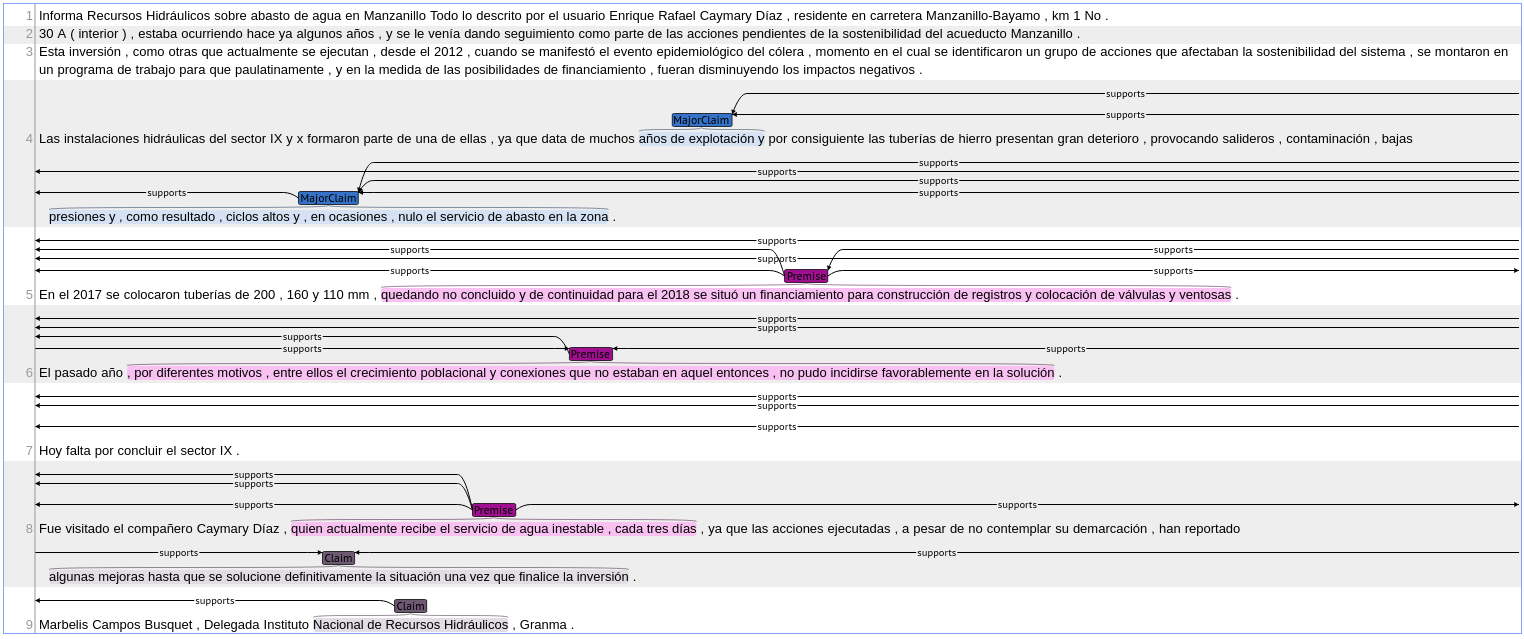
\includegraphics[scale=.4]{Graphics/persuasive_2019-01-25|informa-recursos-hidraulicos-sobre-abasto-de-agua-en-manzanillo|abasto-de-agua-en-manzanillo.png}
		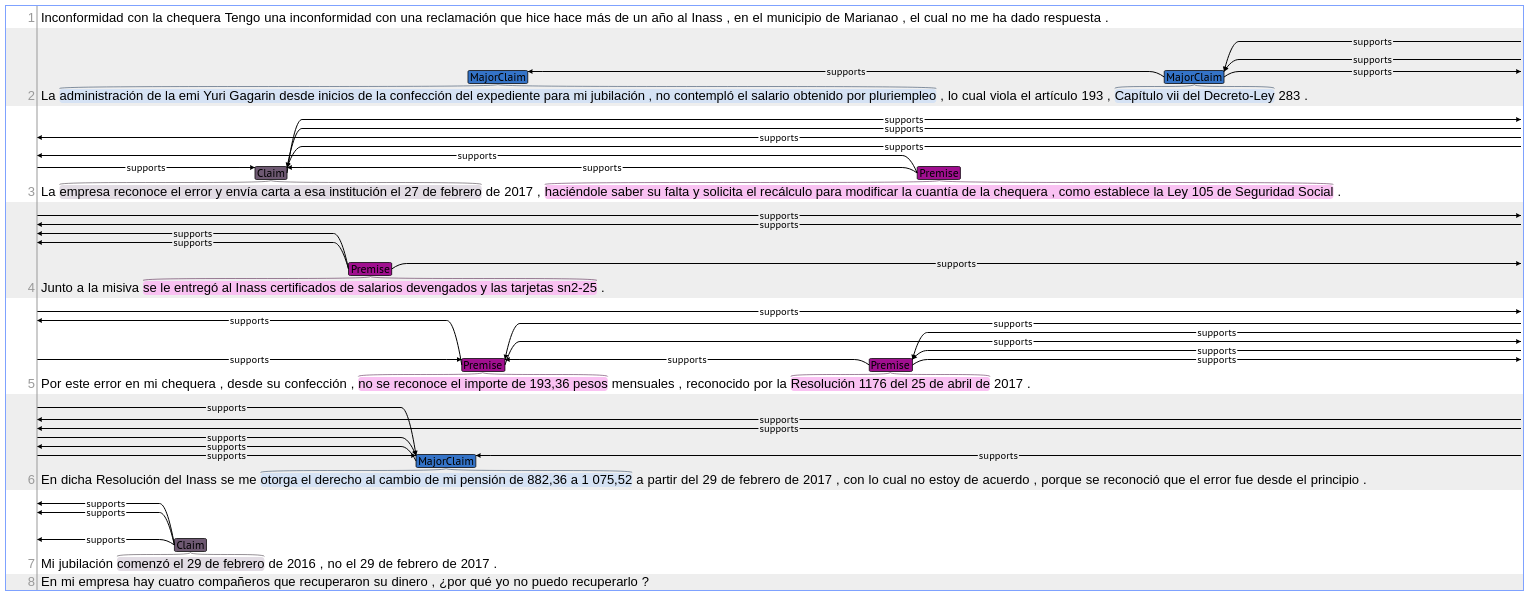
\includegraphics[scale=.4, width=435pt, height=250pt]{Graphics/persuasive_2019-03-22|inconformidad-con-la-chequera.png}
		\caption{Visualización con Brat de las estructuras argumentativas.}\label{fig:brat_persuasive_granma_letters}
	\end{center}
\end{figure}

\subsection{Formato Estándar}

El formato estándar creado es basado en el esquema de anotación CoNLL, donde se anotan a nivel de token todos los aspectos 
relavantes para las tareas a realizar. La segmentación de las UDAs son representadas por las anotaciones 
BIO o BIOES en cada palabra, en adición, las clasificaciones de estas son anotadas al adicionar el nombre 
de esta separada por un guión. Las relaciones son anotadas auxiliándose de la distancia argumentativa, estas 
son agregadas al anotar el tipo de relación con su respectiva distancia ambas separadas por un guión. A 
continuación se muestran ejemplos de este formato, conformado por el token, su clasificación BIOES, su clasificación
UDA, y las relaciones representadas por su clasificación y su distancia argumentativa:

\begin{itemize}
	\item Elemento fuera de una UDA: $análisis \quad O$
	\item UDA intermedia con una relación: $contribuye \quad I-Premise-attacks-5$
	\item Inicio de UDA con dos relaciones: $atletas \quad B-Claim-attacks--1-attacks-12$
\end{itemize}

\section{Experimentación}

Para realizar la selección del modelo se utilizó el corpus de Ensayos Argumentativos. Con este se ajustaron
las arquitecturas e hiperparámetros de los modelos propuestos. La mejor combinación de estos fue utilizada 
para el entrenamiento de los corpus restantes. Finalmente, los modelos fueron utilizados para anotar las Cartas 
a la Dirección. 

\subsection{Hardware}

Gran parte del procesamiento se llevo a cabo en una computadora $i5$ con $8GB$ de RAM ampliada con $4GB$ de memoria 
\emph{swap} [\cite{swap}], aunque se requirió el uso de la plataforma Colab [\cite{colab}] para 
el entrenamiento de algunos modelos por falta de recursos locales.

\subsection{Segmentador de UDA}

En el entrenamiento del segmentador de UDA se hicieron variaciones en la arquitectura propuesta con respecto a la
presencia o no de las siguientes componentes, presentando cuatro candidatos (Tabla \ref{table:segmenter_architecture_table}):

\begin{itemize}
    \item Atributos de POS en la entrada del algoritmo (POS).
    \item Atributos extraídos por la CNN de la palabra (Char-CNN).
    \item Atributos extraídos por la LSTM bidireccional de la palabra (Char-LSTM).
    \item Conexiones residuales (Res).
    \item Capa densa final (Densa).
    \item Capas de normalizaciones (Norm).
\end{itemize}

\begin{table}[h!]
	\begin{center}
		\begin{tabular}{|c|c|c|c|c|c|c|} \hline
		Modelos 		& POS       & Char-CNN  & Char-LSTM & Res       & Norm      & Densa  \\ \hline
		Modelo 1		& $\times$	& $\times$    & $\times$    & $\times$	& $\times$    & $\times$ \\ \hline
		Modelo 2		& $\times$	& $\checkmark$    & $\checkmark$    & $\checkmark$	& $\checkmark$    & $\times$ \\ \hline
		Modelo 3		& $\checkmark$	& $\checkmark$    & $\checkmark$    & $\checkmark$	& $\checkmark$    & $\times$ \\ \hline
		Modelo 4		& $\checkmark$	& $\checkmark$    & $\checkmark$    & $\checkmark$	& $\checkmark$    & $\checkmark$ \\ \hline
		\end{tabular}
	\caption{Variantes de arquitectura de los modelos de segmentación de UDA.}\label{table:segmenter_architecture_table}
	\end{center}
\end{table}

En la Figura \ref{fig:segmenter_model_loss} se observan las diferentes curvas de aprendizaje de los modelos 
probados. Se muestra la rápida convergencia de los modelos con conexiones residuales y normalizaciones.
Se muestra también la tendencia al sobreajuste en el entrenamiento entre los pasos 17-20, en donde se detiene el 
entrenamiento para evitar el crecimiento del error de generalización.

\begin{figure}[h!]
	\begin{center}
		\begin{center}
			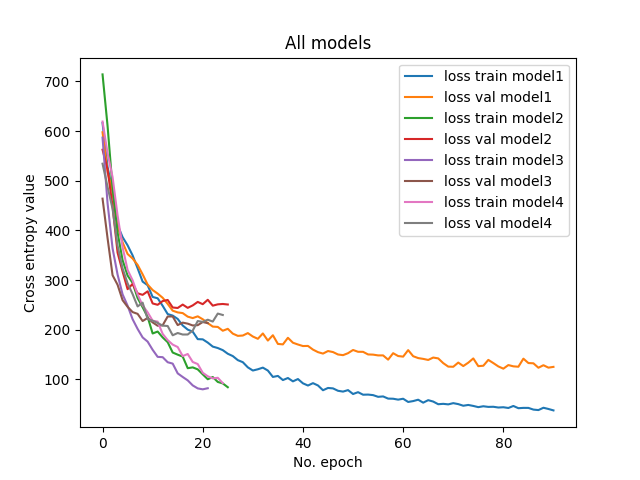
\includegraphics[scale=.7]{Graphics/persuasive_essays_all_linked_crf_loss.png}
        \end{center}
	    \caption{Pérdida de los modelos segmentadores.}\label{fig:segmenter_model_loss}
	\end{center}
\end{figure}

Las métricas 100\%F1 y 50\%F1 muestran que los modelos 1 y 2 presentan un desempeño menor que los 3 y 4. 
Se muestra un ligero aumento de 1\% en las 50\%F1 en el modelo 4 con respecto 
al modelo 3, aunque las métricas de F1 en el 3 superan a las de 4. Se considera a la 
segmentación como tarea principal, por lo que se selecciona como mejor modelo al 4 (Figura \ref{fig:test_segmenter_model_metrics}).
Las distinciones BIOES en los nombres de tablas o métricas constituyen la métricas correspondientes 
a la segmentación estrictamente, mientras las que no poseen dicha distinción sontituye al proceso 
conjunto de segmentación y clasificación de UDAs. 

\begin{figure}[h!]
	\begin{center}
		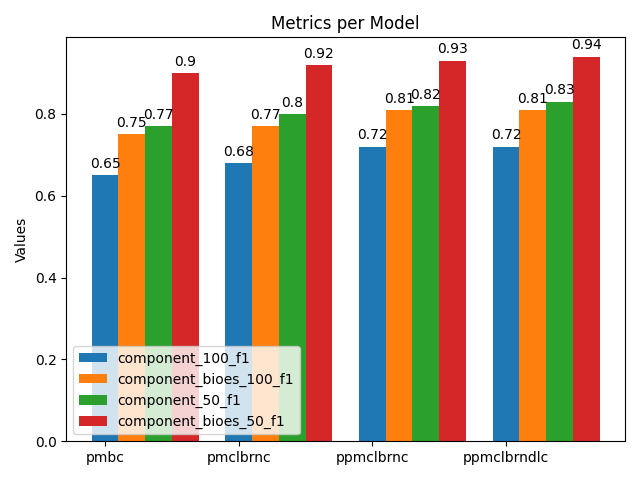
\includegraphics[scale=.4]{Graphics/persuasive_essays_all_linked_components.png}
		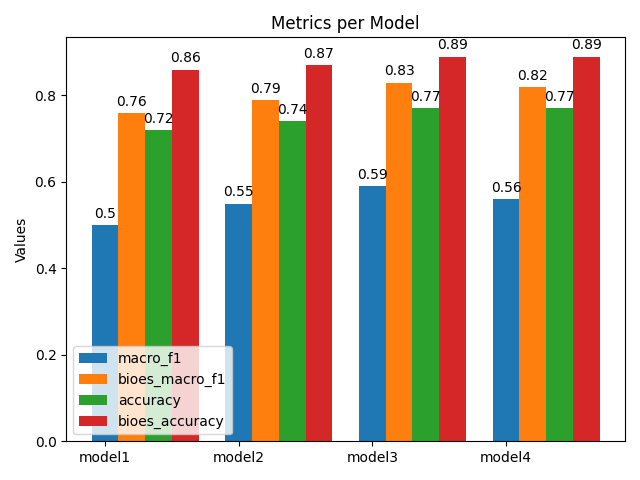
\includegraphics[scale=.4]{Graphics/persuasive_essays_all_linked_macro_micro_metrics.png}
	    \caption{Métricas del conjunto de pruebas de los modelos segmentadores.}\label{fig:test_segmenter_model_metrics}
	\end{center}
\end{figure}

El modelo seleccionado fue usado en el entrenamiento de los demás conjuntos de datos obteniendo los resultados mostrados
en Tabla \ref{table:test_metrics_segmenter} y Tabla \ref{table:test_bioes_metrics_segmenter}.

\begin{table}[h!]
	\begin{center}
		\scalebox{0.9}{
		\begin{tabular}{|c|c|c|c|c|c|} \hline
        Corpus		            & F1 Ponderado  & Macro F1	& \emph{Accuracy} & 100\%F1 & 50\%F1  	   \\ \hline
        Ensayos Argumentativos  & 0,76          & 0,56 		& 0,77		      & 0,72    & 0,83       \\ \hline
        CDCP		            & 0,65          & 0,45 		& 0,66		      & 0,61    & 0,68       \\ \hline
        AbsTRCT	                & 0,86          & 0,50 		& 0,87		      & 0,61    & 0,75       \\ \hline
        \end{tabular}
		}
	\caption{Métricas de las pruebas del segmentador de UDA.}\label{table:test_metrics_segmenter}
	\end{center}
\end{table}
\begin{table}[h!]
	\begin{center}
		\scalebox{0.9}{
		\begin{tabular}{|c|c|c|c|c|c|} \hline
        Corpus		            & F1 Ponderado  & Macro F1 & \emph{Accuracy} & 100\%F1 &  50\%F1   \\ \hline
        Ensayos Argumentativos  & 0,89          & 0,82	   & 0,89            & 0,81	   & 0,94 	   \\ \hline
        CDCP		            & 0,95          & 0,56	   & 0,96	         & 0,82	   & 0,93 	   \\ \hline
        AbsTRCT	                & 0,90          & 0,79	   & 0,91	         & 0,66	   & 0,82 	   \\ \hline
        \end{tabular}
		}
	\caption{Métricas BIOES de las pruebas del segmentador de UDA.}\label{table:test_bioes_metrics_segmenter}
	\end{center}
\end{table}

\subsection{Predictor de Enlaces}

Para el modelo se realizó un voto conjunto del ensamblado de 3 modelos, dado que el entrenamiento 
está basado en la aleatoriedad, se entrenan los modelos con los mismos datos obteniendo inferencias no
necesariamente iguales.
Para la selección del modelo se entrenaron diferentes variantes de arquitecturas e hiperparámetros, y 
al igual que en el segmentador de UDAs se realizó la selección del modelo que mejor se desempeñó en 
el conjunto de datos de Ensayos Argumentativos. De las variaciones surgieron las siguientes propuestas
(Tabla \ref{table:link_predictor_architecture_table}):

\begin{table}[h!]
	\begin{center}
		\scalebox{0.85}{
		\begin{tabular}{|c|c|c|c|c|c|c|} \hline
		Modelos   	 & Atención      & Pooling  & \emph{Dropout}   & Tasa de aprendizaje & Paciencia & Devolver mejores     \\ \hline
		Modelo 1	 & $\times$	     &  5       & 0,5               & 0,0015               & 10	      & $\checkmark$        \\ \hline
		Modelo 2	 & $\times$	 	 & 10       & 0,1               & 0,003                & 5	      & $\times$            \\ \hline
		Modelo 3	 & $\checkmark$	 &  1       & 0,1               & 0,003                & 5	      & $\times$            \\ \hline
		Modelo 4	 & $\checkmark$	 &  1       & 0,5               & 0,0015               & 10	      & $\checkmark$        \\ \hline
		\end{tabular}
		}
	\caption{Variantes de arquitectura de los modelos de predicción de enlaces.}\label{table:link_predictor_architecture_table}
	\end{center}
\end{table}

Las curvas de aprendizaje del proceso de entrenamiento de los modelos (Figura \ref{fig:link_prediction_model_loss}) 
muestran un nivel de sobreajuste 
elevado que disminuyen cuando el \emph{dropout} aumenta. Además, se observan valores de pérdida elevados lo que significa 
que al modelo le cuesta ajustarse de manera satisfactoria a los datos.

\begin{figure}[h!]
	\begin{center}
		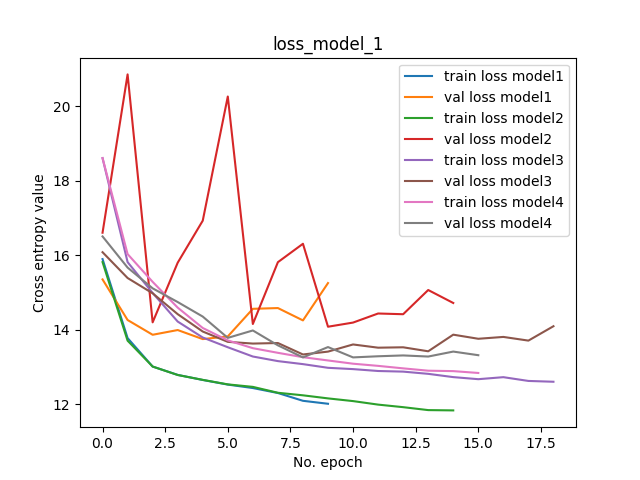
\includegraphics[scale=.7]{Graphics/persuassive_essays_all_linked_link_prediction_loss_model_1.png}
	    \caption{Curvas de aprendizaje de los modelos de predicción de enlaces.}\label{fig:link_prediction_model_loss}
	\end{center}
\end{figure}

Las métricas obtenidas por las diferentes versiones de los modelos 
(Figura \ref{fig:link_prediction_model_metrics}) 
muestran que el modelo 2 constituye una opción ligeramente superior en lo correspondiente a 
predicción de enlace a los otros modelos. Esos hiperparámetros
fueron utilizados para el entrenamiento con los demás conjuntos de datos.

\begin{figure}[h!]
	\begin{center}
		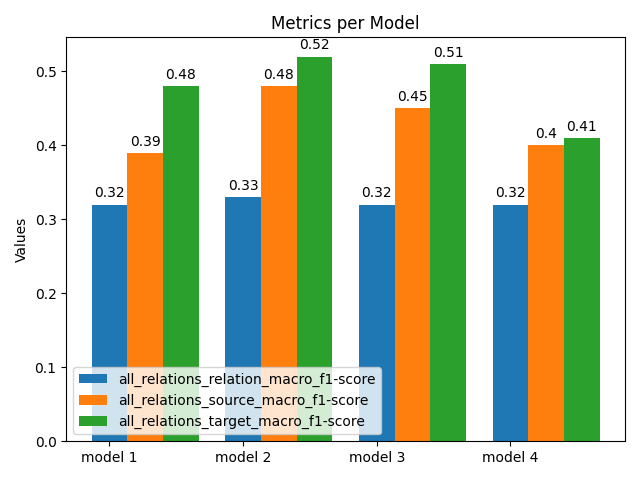
\includegraphics[scale=.4]{Graphics/persuasive_essays_all_linked_all_relation_f1_scores.png}
		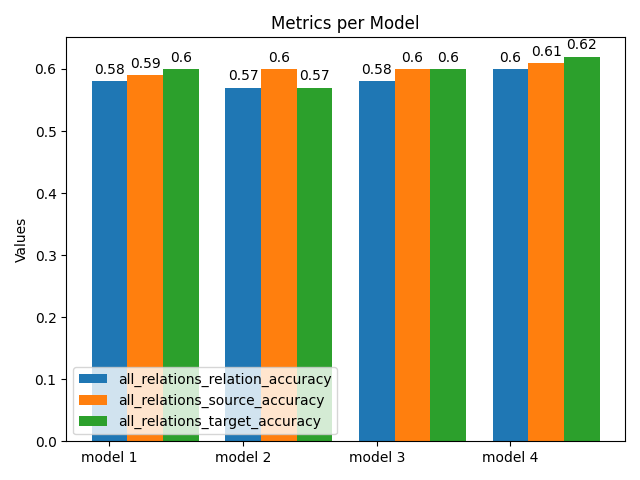
\includegraphics[scale=.4]{Graphics/persuasive_essays_all_linked_all_relation_accuracy.png}\\
		\text{a)$\qquad \qquad \qquad \qquad \qquad \qquad \qquad \qquad $b)}
	\end{center}
	\begin{center}
		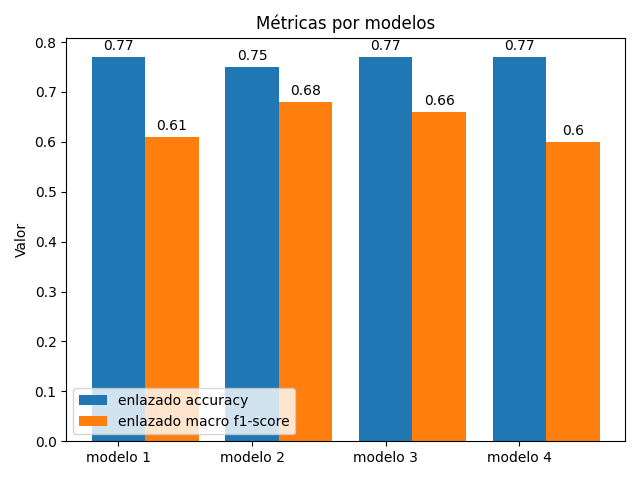
\includegraphics[scale=.4]{Graphics/persuasive_essays_all_linked_all_relation_linked.png}\\
		\text{c)}
	\end{center}
	\caption{Métricas F1 de la clasificación de enlace (a), \emph{accuracy} (b) y
			F1 de la predicción de enlace (c) de los modelos de predicción de enlaces.}
	\label{fig:link_prediction_model_metrics}
\end{figure}

En el entrenamiento del modelo en los demás conjuntos de datos se obtuvieron los resultados de las Tablas 
\ref{table:test_relation_metrics_link_predictor} y \ref{table:test_source_metrics_link_predictor}.

\begin{table}[h!]
	\begin{center}
		\scalebox{0.9}{
		\begin{tabular}{|c|c|c|c|c|} \hline
        Corpus		            & Macro F1 & \emph{Accuracy} & Macro F1 Enlace  & \emph{Accuracy} Enlace  \\ \hline
        Ensayos Argumentativos  & 0,33	   & 0,57            & 0,68	    		& 0,75	    		  	  \\ \hline
        CDCP		            & 0,37	   & 0,63	         & 0,79	    		& 0,68	    		  	  \\ \hline
        AbsTRCT	                & 0,39	   & 0,61	         & 0,83	    		& 0,74	    		  	  \\ \hline
        \end{tabular}
		}
	\caption{Métricas de predicción de relaciones de las pruebas del predictor de enlace.}\label{table:test_relation_metrics_link_predictor}
	\end{center}
\end{table}

\begin{table}[h!]
	\begin{center}
		\begin{tabular}{|c|c|c|c|} \hline
        Corpus		            & F1 Macro  & \emph{Accuracy} \\ \hline
        Ensayos Argumentativos  & 0,48       & 0,60             \\ \hline
        CDCP		            & 0,26       & 0,52	         \\ \hline
        AbsTRCT	                & 0,51       & 0,79	         \\ \hline
        \end{tabular}
	\caption{Métricas de predicción de fuente de las pruebas del predictor de enlace.}\label{table:test_source_metrics_link_predictor}
	\end{center}
\end{table}

\begin{table}[h!]
	\begin{center}
		\begin{tabular}{|c|c|c|c|} \hline
        Corpus		            & Macro F1 & \emph{Accuracy} \\ \hline
        Ensayos Argumentativos  & 0,52	   & 0,57             \\ \hline
        CDCP		            & 0,36	   & 0,54	         \\ \hline
        AbsTRCT	                & 0,53	   & 0,81	         \\ \hline
        \end{tabular}
	\caption{Métricas de predicción de objetivo de las pruebas del predictor de enlace.}\label{table:test_target_metrics_link_predictor}
	\end{center}
\end{table}

\subsection{Acoplamiento de los modelos}

Dado que la clasificación de UDAs es hecha tanto en el segmentador como en el predictor de enlaces, es necesaria 
la selección de cómo se va a desambiguar esta clasificación. En caso de seleccionar el predictor de enlaces como 
clasificador final, surgen varias cuestiones, como por ejemplo, que las UDAs pueden tomar varias clasificaciones o el
predictor no toma el contexto del texto completo en la clasificación. Aunque la primera puede ser corregida
mediante la selección de la clase más votada o algún otro criterio, la segunda presenta un mayor problema. Por
esto es seleccionada la clasificación del segmentador como etiqueta final para las UDAs y el predictor es usado para 
la tarea de extracción y clasificación de relaciones.

\subsection{Comparación con el estado del arte}

Las comparaciones se realizan por conjuntos de datos y se muestran las 
métricas indicadas por los autores de cada propuesta. Cada corpus y propuesta 
presenta características únicas que hacen que comparaciones directas sean 
difíciles de realizar, por lo tanto, la información brindada muestra una comparación 
cualitativa y no cuantitativa en la mayoría de los casos. 

Una de las principales dificultades está dada por el hecho de que las métricas calculadas son de la versión proyectada
al español, lo cual contribuye a variaciones en las etiquetas finales debido al lenguaje mismo 
o a errores en el proceso. Otros ejemplos en la dificultad de comparar las métricas se encuentra
en los enfoques tomados por las investigaciones anteriores a la hora de realizar las tareas.
En algunos casos la segmentación se presenta como una tarea de clasificación BIO, o simplemente 
se separan por oraciones y las clasifican en argumentativas o no. En el aspecto de clasificación
de las UDAs se emplean métodos como su clasificación independiente luego de ser extraída o su modelación
conjunta con la segmentación. En la extracción y clasificación de relaciones se observan técnicas de 
optimización de problemas enteros, clasificación por SVM o también probando los posibles enlaces dos 
a dos independientemente.

En la comparación de métodos se seleccionaron seis métricas que evalúan las diferentes 
tareas de la EA. La métrica BIOES F1 se refiere 
a la Macro F1 de la clasificación de las etiquetas BIOES, esta constituye una medida
que califica la tarea de segmentación de UDAs en el texto. La métrica Clas UDA F1 es 
calculada como la Macro F1 de las etiquetas BIOES junto con las etiquetas del tipo de 
UDA, medida que evalúa la tarea de clasificación de las UDAs. Rel Pred F1 es la medida 
Macro F1 de la predicción de enlaces y Rel Clas F1 la de la clasificación, estas 
son calculadas tomando en cuenta todos los pares seleccionados para el conjunto de 
datos. En la comparación $\checkmark$ significa que son directamente comparables,
$*$ que el método de comparación es el mismo, pero no son usados los mismos 
elementos para calcular la métrica, y $\times$ que la métrica no se encontraba disponible.

\begin{table}[h!]
	\begin{center}
		\scalebox{0.85}{
		\begin{tabular}{|c|c|c|c|c|c|} \hline
		Corpus		            & Propuesto  & \cite{stab2017parsing} & \cite{niculae2017argument} & \cite{galassi2021deep} \\ \hline
		BIOES F1 				& 0,82   	 & 0,85 $\checkmark$	  & $\times$        	       & $\times$				\\ \hline
		Clas UDA F1		        & 0,56	     & 0,82        			  & 0,77	    			   & 0,53					\\ \hline
		Rel Pred F1 			& 0,68   	 & 0,58        			  & 0,60			    	   & 0,36 *				   	\\ \hline
		Rel Clas F1 			& 0,33   	 & 0,70        			  & $\times$	    	       & 0,18 *				   	\\ \hline
		\end{tabular}
		}
	\caption{Métricas comparativas de Ensayos Persuasivos.}\label{table:comparative_test_essays_f1_metrics_segmenter}
	\end{center}
\end{table}
\begin{table}[h!]
	\begin{center}
		\begin{tabular}{|c|c|c|c|c|c|} \hline
		Corpus		            & Propuesto  & \cite{niculae2017argument} & \cite{galassi2021deep}  \\ \hline
		BIOES F1 				& 0,56  	 & $\times$        	       	  & $\times$				\\ \hline
		Clas UDA F1		        & 0,45	     & 0,73 				 	  & 0,79					\\ \hline
		Rel Pred F1				& 0,68   	 & 0,27			    	      & 0,30	*			   	\\ \hline
		Rel Clas F1				& 0,37   	 & $\times$	    	          & 0,15	*			   	\\ \hline
		\end{tabular}
	\caption{Métricas comparativas de CDCP.}\label{table:comparative_test_cdcp_f1_metrics_segmenter}
	\end{center}
\end{table}
\begin{table}[h!]
	\begin{center}
		\begin{tabular}{|c|c|c|c|c|c|} \hline
		Corpus		            & Propuesto  & \cite{mayer2020transformer} & \cite{galassi2021deep} \\ \hline
		BIOES F1 				& 0,79   	 & $\times$   				   & $\times$				\\ \hline
		Clas UDA F1		        & 0,50	     & 0,88	$\checkmark$		   & 0,91					\\ \hline
		Rel Pred F1 			& 0,74   	 & $\times$	   				   & 0,54 *				   	\\ \hline
		Rel Clas F1 			& 0,39   	 & 0,66  *	   				   & 0,70 *				   	\\ \hline
		\end{tabular}
	\caption{Métricas comparativas de AbsTRCT.}\label{table:comparative_test_abstrct_f1_metrics_segmenter}
	\end{center}
\end{table}

\section{Validación}

Dado que las estructuras argumentativas varían en su forma en cada corpus es complejo realizar un método que evalúe de forma 
justa los resultados obtenidos por los diferentes modelos de manera conjunta. Una variante sería anotar las cartas 
con los esquemas argumentativos presentes en los conjuntos de datos, esto constituye una labor en la que se requiere
personal experto y previo estudio y preparación, además de tiempo. El proceso que se lleva a cabo para realizar la 
validación consiste en un análisis cualitativo realizado a criterio del autor. Para esto se seleccionaron 15 pares 
de cartas, la carta original y la respuesta enviada a esta. Cada uno de estas 30 cartas fueron anotadas por los modelos entrenados en cada 
conjunto de datos y se realizó el análisis de calidad correspondiente. Los puntos por los que se llevó a cabo el análisis
se resumen en los siguientes:

\begin{itemize}
	\item ¿La UDA se extrajo correctamente?
	\item ¿La UDA se clasificó correctamente?
	\item ¿La relación se extrajo correctamente?
	\item ¿La relación se clasificó correctamente?
\end{itemize}

% \begin{itemize}
% 	\item Muchos falsos positivos en la predicción de enlaces, debido a la manera en la manera componente a componente que 
% 	se hacen
% 	\item En los textos en donde la segmentación es por oraciones, los puntos relacionados a otra acción que 
% 	no sea separar oraciones son seleccionados como separadores.
% 	\item La segmentación, se queda corta o larga?
% \end{itemize}

\subsection{Análisis de Ensayos Argumentativos}

% \begin{figure}[h!]
% 	\begin{center}
% 		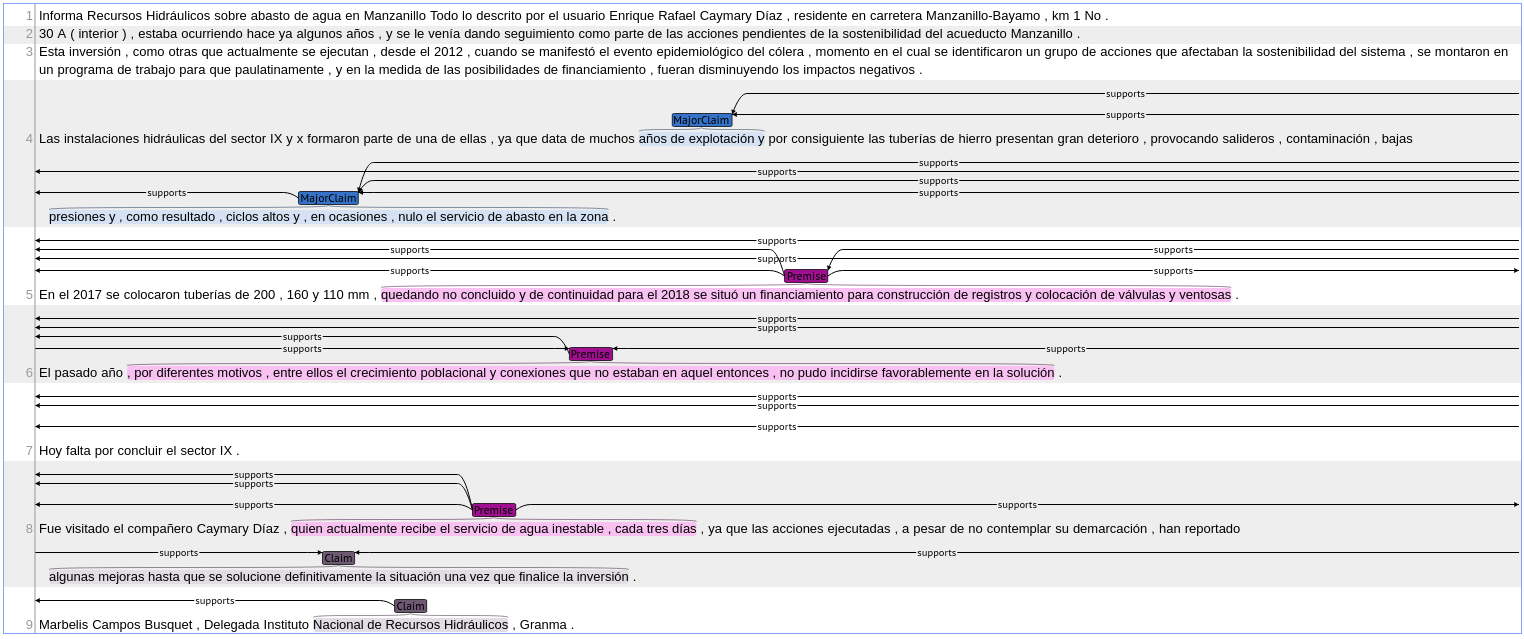
\includegraphics[scale=.4]{Graphics/persuasive_2019-01-25|informa-recursos-hidraulicos-sobre-abasto-de-agua-en-manzanillo|abasto-de-agua-en-manzanillo.png}
% 		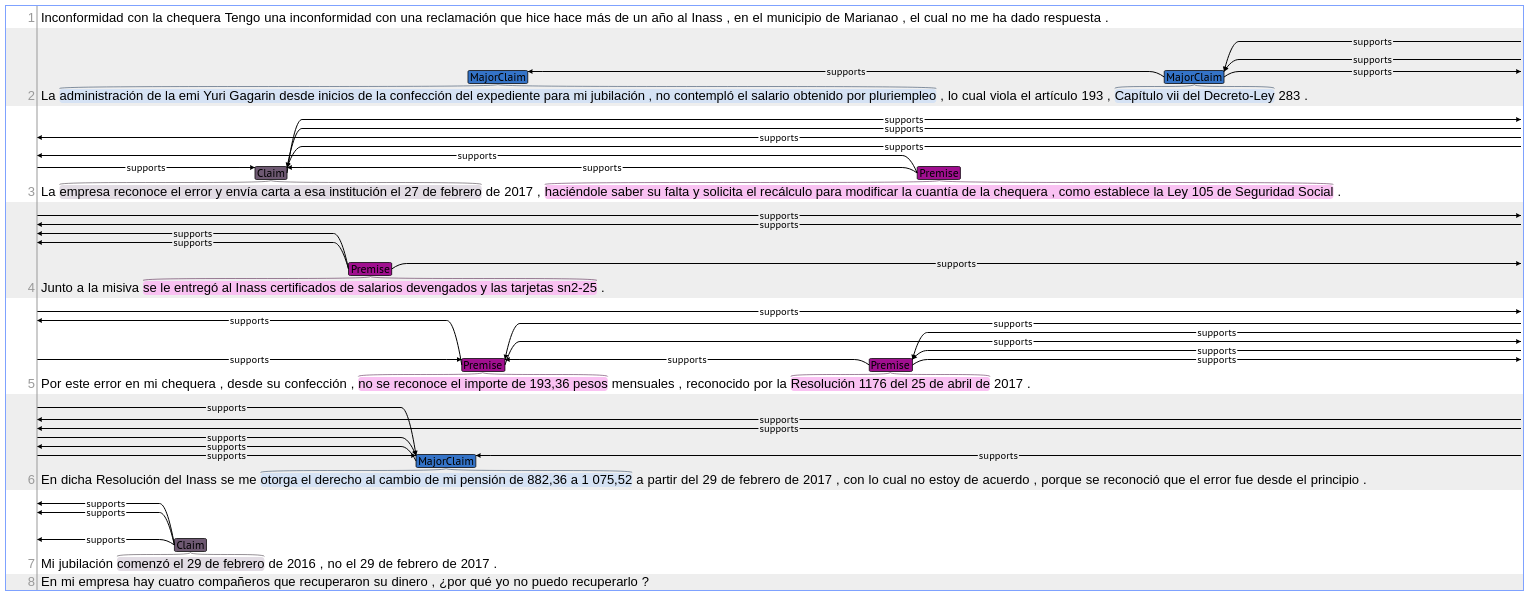
\includegraphics[scale=.4]{Graphics/persuasive_2019-03-22|inconformidad-con-la-chequera.png}
% 	    \caption{A}\label{fig:persuasive_granma_letters}
% 	\end{center}
% \end{figure}

Los ensayos argumentativos presentan una anotación de UDAs a un nivel de unidades de texto que pueden ser 
más pequeñas que oraciones y clasifican estas en las clases \emph{MajorClaim} (MC), \emph{Claim} (C) y \emph{Premise} 
(P). Las relaciones se clasifican en de \emph{supports} y \emph{attacks}. 

En general, se observa que se presentan problemas en la segmentación de UDAs debido al formato y dominio del texto.
Las cartas presentan una estrutura en donde al final se realiza una firma poniendo información acerca del remitente,
esta estructura no contribuye a la argumentación, pero el modelo en varias ocasiones detecta componentes en estas. 
Además de estos problemas de la estructura característica de la carta se encuentran otros. Entre los más 
encontrados se observa la extracción de supuestas UDAs que en su contenido no se encuentra un componente argumentativo, 
generalmente, estos elementos, si se expanden, pueden lograr establecer una mejor UDA.

Ejemplos malos:
\begin{itemize}
	\item \text{} [años de explotación y]$_{MC}$ 
	: Muy corto y no informativo. % 2019-01-25|informa-recursos-hidraulicos-sobre-abasto-de-agua-en-manzanillo|abasto-de-agua-en-manzanillo.txt.conll.link.conll.ann
	\item \text{} [en cada uno de los establecimientos de nuestra Cadena de Tiendas]$_{MC}$ 
	: Incompleto, mejora incorporando elementos de la izquierda (No a todos los productos con próxima fecha de vencimiento se le aplica rebaja de precios). % 2018-12-07|responde-trd-caribe-al-consumidor|a-proposito-de-la-proteccion-al-consumidor.txt.conll.link.conll.ann
	\item \text{} [Director División Grandes Centros]$_{MC}$ [TRD Caribe]$_{C}$ 
	: Mala clasificación y segmentación. %  2018-12-07|responde-trd-caribe-al-consumidor|a-proposito-de-la-proteccion-al-consumidor.txt.conll.link.conll.ann
	\item \text{} [Esperamos lo antes posible una solución]$_{P}$ 
	: En contexto, no contiene información que lo haga premisa % 2018-10-05|abasto-de-agua-en-manzanillo.txt.conll.link.conll.ann
	\item \text{} [no podemos permitir]$_{C}$ 
	: No establece una \emph{claim} % 2017-06-30|inass-reconoce-razon-de-ramiro-castellanos-por-inconformidad-con-trato-de-especialista-de-las-tunas|pregunta-quien-le-paga-su-jubilacion.txt.conll.link.conll.ann
\end{itemize}

Ejemplos buenos:
\begin{itemize}
	\item \text{} [no se le puede volver a despachar, tiene que ver a la administración (si está ahí en ese momento), 
	si no, regresar al día siguiente para que se le acredite lo sucedido]$_{MC}$ % 2021-02-26|inconvenientes-con-tarjetas-de-combustible-en-moneda-nacional.txt.conll.link.conll.ann
	\item \text{} [administración de la EMI Yuri Gagarin desde inicios de la confección del expediente para 
	mi jubilación, no contempló el salario obtenido por pluriempleo]$_{MC}$ % 2019-03-22|inconformidad-con-la-chequera.txt.conll.link.conll.ann
	\item pudiese [contribuir al ahorro de agua y la prestación de un mejor servicio]$_C$ % 2018-10-05|abasto-de-agua-en-manzanillo.txt.conll.link.conll.ann
	\item \text{} [es que estamos limitados de este servicio, y no desde hace un tiempo, es que nunca lo hemos tenido]$_P$ % 2018-05-18|sin-cobertura-en-guara-mayabeque.txt.conll.link.conll.ann
	\item \text{} [el número de carné de identidad que se encontraba en dicha base de datos correspondía a otra persona que
	fue reportada como fallecida]$_P$ % 2017-06-30|inass-reconoce-razon-de-ramiro-castellanos-por-inconformidad-con-trato-de-especialista-de-las-tunas|pregunta-quien-le-paga-su-jubilacion.txt.conll.link.conll.ann
\end{itemize}

Las relaciones anotadas por el modelo tienden a contener una gran cantidad de falsos positivos, además
dado que este conjunto de datos posee un gran desbalance en las etiquetas de las relaciones favoreciendo 
estas a las de \emph{supports}, el modelo no fue capaz de realizar anotaciones de \emph{attacks}, tanto en 
el conjunto de original de pruebas como en las cartas.

\subsection{Análisis de CDCP}

% \begin{figure}[h!]
% 	\begin{center}
% 		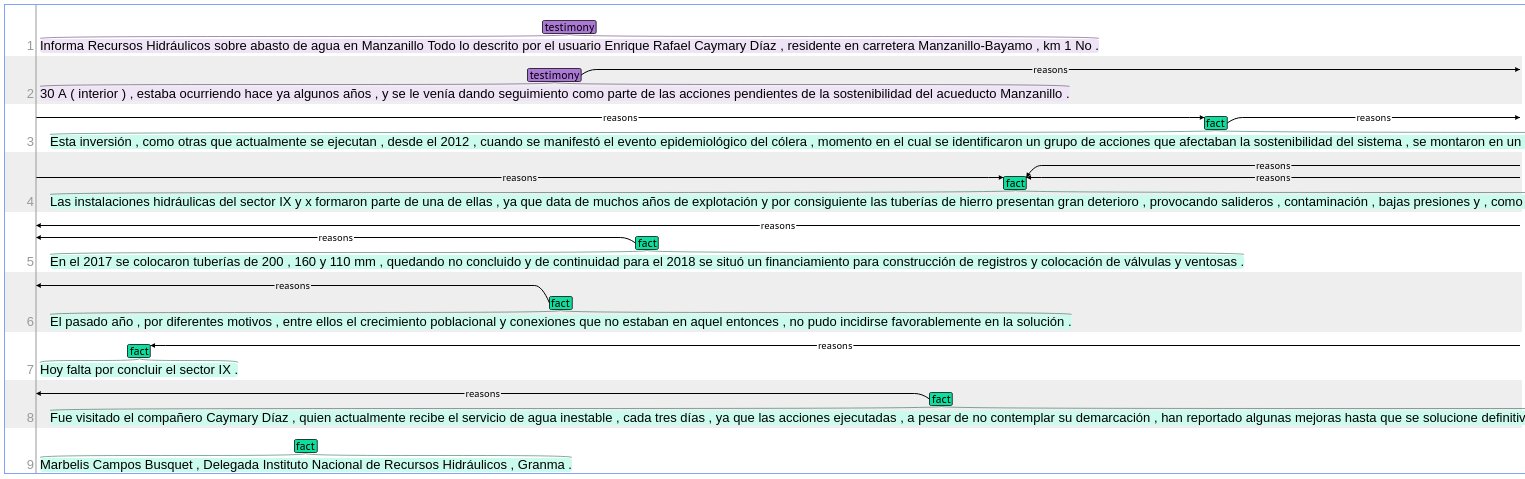
\includegraphics[scale=.4]{Graphics/cdcp_2019-01-25|informa-recursos-hidraulicos-sobre-abasto-de-agua-en-manzanillo|abasto-de-agua-en-manzanillo.png}
% 		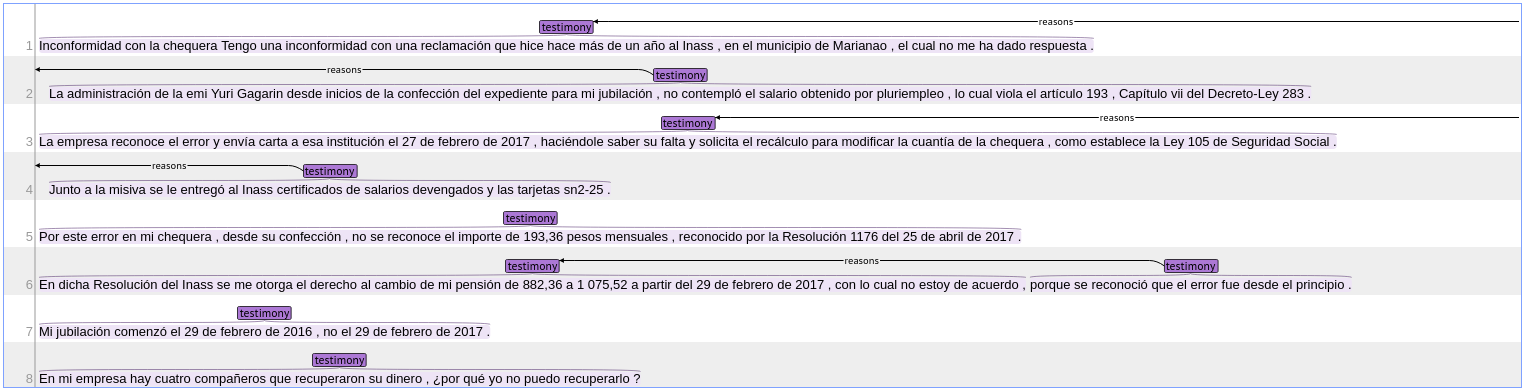
\includegraphics[scale=.4]{Graphics/cdcp_2019-03-22|inconformidad-con-la-chequera.png}
% 	    \caption{A}\label{fig:cdcp_granma_letters}
% 	\end{center}
% \end{figure}

CDCP realiza la segmentación de UDAs en la mayoría de las situaciones al separarlas por oraciones 
(solamente el 1\% de los tokens se encuentran fuera de una UDA),
estas son clasificadas en \emph{testimony} (T), \emph{fact} (F), \emph{policy} (P), \emph{reference} (R)
y \emph{value} (V). Las relaciones presentan dos tipos de relaciones \emph{evidences} y \emph{reasons}.

Los errores más comunes cometidos en la segmentación, dado el esquema utilizado, provienen del uso 
de signos de puntuación que no representan un cambio de oración, en estos casos se separa las UDA. También
existen errores de clasificación incorrecta, de, por ejemplo, \emph{testimony} que podrían ser \emph{fact}.

Ejemplos malos:
\begin{itemize}
	\item \text{} [\dots Bayamo, km 1 No.]$_T$ [30 A (interior), \dots]$_T$ 
	: Uso del \textbf{.} para abreviar número se toma como separador de UDA. % 2019-01-25|informa-recursos-hidraulicos-sobre-abasto-de-agua-en-manzanillo|abasto-de-agua-en-manzanillo.txt.conll.link.conll.ann
	\item \text{} [\dots ,desde el 1ro.]$_T$ [de marzo \dots]$_T$ 
	: Uso del \textbf{.} para abreviar primero se toma como separador de UDA. % 2019-05-24|le-retribuyen-la-diferencia-reclamada-de-su-pension|inconformidad-con-la-chequera.txt.conll.link.conll.ann
	\item \text{} [Junto a la misiva se le entregó al Inass certificados de salarios devengados y las tarjetas sn2-25.]$_T$ 
	: Se clasifica mejor como \emph{fact}. % 2019-03-22|inconformidad-con-la-chequera.txt.conll.link.conll.ann
	\item \text{} [Caridad Real Gutiérrez, Jefe de Trámites y Pensiones, Inass.]$_T$ 
	: Firma de la carta como elemento argumentaivo. % 2019-05-24|le-retribuyen-la-diferencia-reclamada-de-su-pension|inconformidad-con-la-chequera.txt.conll.link.conll.ann
\end{itemize}

Ejemplos buenos:
\begin{itemize}
	\item \text{} [En el 2017 se colocaron tuberías de 200, 160 y 110 mm, quedando no concluido y de 
	continuidad para el 2018 se situó un financiamiento para construcción de registros y colocación de 
	válvulas y ventosas.]$_F$ % 2019-01-25|informa-recursos-hidraulicos-sobre-abasto-de-agua-en-manzanillo|abasto-de-agua-en-manzanillo.txt.conll.link.conll.ann
	\item \text{} [Mi jubilación comenzó el 29 de febrero de 2016, no el 29 de febrero de 2017.]$_T$ % 2019-03-22|inconformidad-con-la-chequera.txt.conll.link.conll.ann
	\item \text{} [No se sabe cuánto queda, lo que obliga al cliente a estar haciendo cuentas constantemente.]$_F$ % 2021-05-07|servicentros-operan-diversos-medios-de-pago-electronicos|inconvenientes-con-tarjetas-de-combustible-en-moneda-nacional.txt.conll.link.conll.ann
\end{itemize}

Las relaciones presentes disminuyen en cantidad en comparación con lo visto en los textos anotados con el modelo 
entrenado con Ensayos Argumentativos. Prevaleciendo las relaciones de \emph{reasons}. A consideración del autor,
la cantidad de los falsos positivos son menores que el modelo de Ensayos Argumentativos.

\subsection{Análisis AbsTRCT}

% \begin{figure}[h!]
% 	\begin{center}
% 		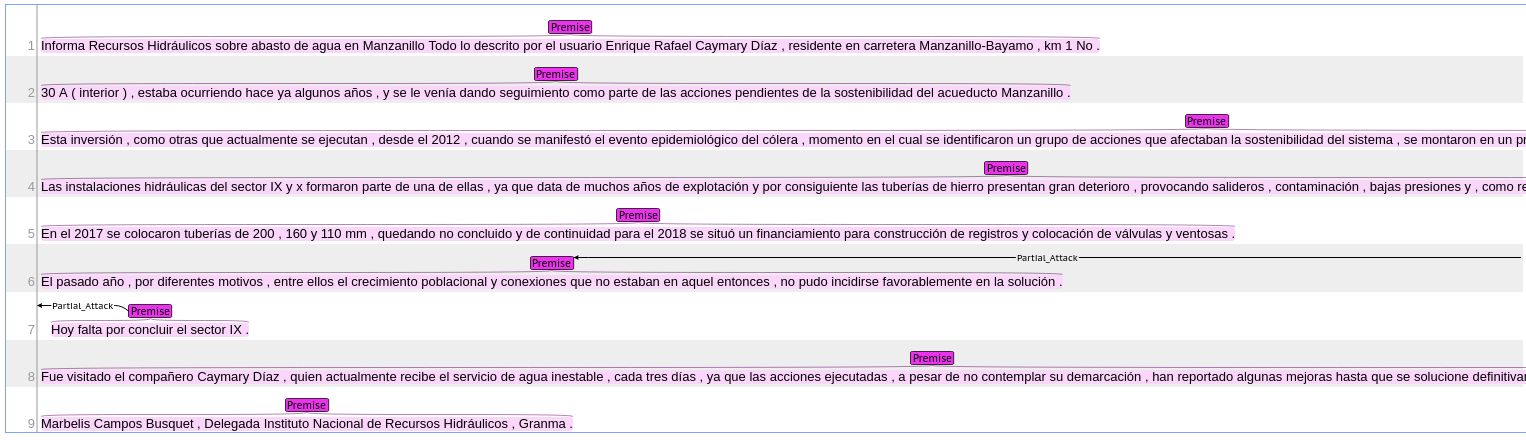
\includegraphics[scale=.4]{Graphics/abstrct_2019-01-25|informa-recursos-hidraulicos-sobre-abasto-de-agua-en-manzanillo|abasto-de-agua-en-manzanillo.png}
% 		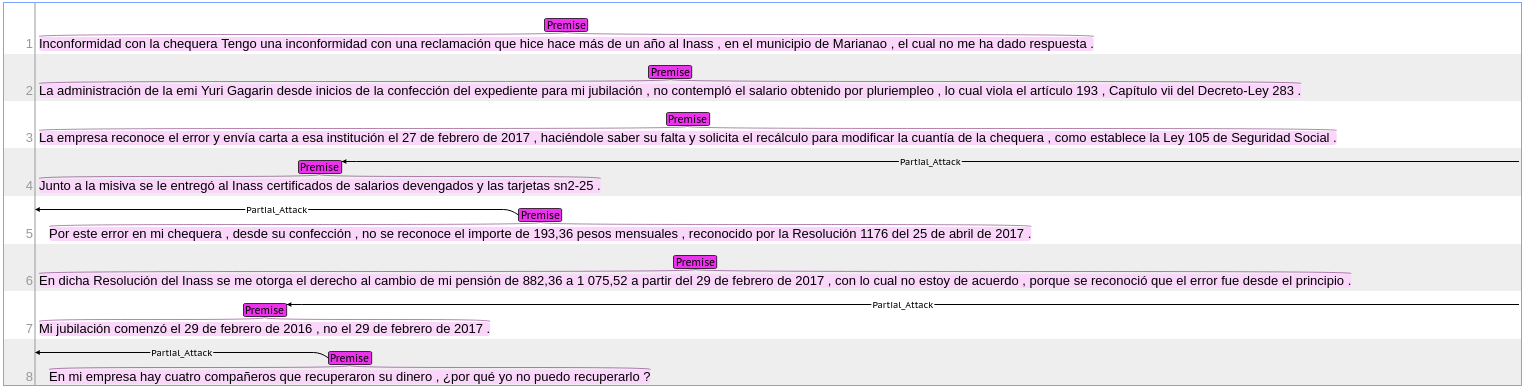
\includegraphics[scale=.4]{Graphics/abstrct_2019-03-22|inconformidad-con-la-chequera.png}
% 		\caption{A}\label{fig:abstrct_granma_letters}
% 	\end{center}
% \end{figure}

El conjunto de datos presenta un estilo de segmentación de UDAs en donde se anotan 
secciones de textos más grandes que en Ensayos Argumentativos, aunque no necesariamente 
todas las oraciones o la oración completa es considerada argumentativa. 
Estas se clasifican igual que Ensayos Argumentativos, aunque 
en este conjunto de datos se presenta un desbalance de etiquetas grande, favoreciendo 
a las \emph{Premise} y las \emph{Claim}, dejando sin representación casi a \emph{MajorClaim}
(menor del 1\% de las etiquetas BIOES), lo que trajo como consecuencia que el modelo no fuera 
capaz de diferenciar este tipo de UDA. Las relaciones se presentaron como \emph{partial-attack},
\emph{attack} y \emph{support}, influenciadas también por la poca cantidad de relaciones de \emph{attack}.

En la clasificación de UDAs se evidencia una gran cantidad de \emph{Premise}.

Ejemplos malos:
\begin{itemize}
	\item \text{} [\dots Calle 14, apto.]$_P$ [4 entre Zapata y 23, \dots]$_T$ 
	: Uso del \textbf{.} para abreviar apartamento se toma como separador de UDA. % 2017-07-07|parque-en-pleno-deterioro-en-plaza.txt.conll.link.conll.ann
	\item \text{} [, Director División Grandes Centros TRD Caribe.]$_C$ 
	: Mala clasificación con mala segmentación y detección de \emph{claim} en firma de carta. 
\end{itemize}

Ejemplos buenos:
\begin{itemize}
	\item \text{} [Esta situación pudo haberse evitado y no podemos permitir que hechos como este ocurran pues, 
	empañan la imagen de la institución que está destinada a brindar un servicio con calidad a la población en 
	general y en especial a los jubilados y pensionados.]$_P$ % 2017-06-30|inass-reconoce-razon-de-ramiro-castellanos-por-inconformidad-con-trato-de-especialista-de-las-tunas|pregunta-quien-le-paga-su-jubilacion.txt.conll.link.conll.ann
	\item \text{} [Esta respuesta considera sin razón la preocupación de un lector, 
	¿así debe terminar la inquietud de un ciudadano, que confía en las instituciones con que cuenta la 
	sociedad para enfrentar sus problemas?]$_C$ % 2017-05-12|cimex-se-dirige-a-limitado-fisico-motor|llamado-a-evaluar-situacion-de-piezas-y-baterias-para-equipos-motorizados-de-discapacitados.txt.conll.link.conll.ann
\end{itemize}

Las relaciones tienen la menor cantidad de elementos de los otros conjuntos de datos, proliferando
las relaciones de \emph{support}. En las clasificadas como \emph{partial-attack} se evidenció, a 
consideración del autor, una baja precisión. Por ejemplo 
[\emph{cierto que la responsabilidad es de todos, pero la institucional es de la Dirección de Comunales.}]
ataca a [\emph{Antonio Blanco, Director de Servicios Comunales Plaza,}].

\subsection{Resultados}

Se considera que el conjunto de datos CDCP se ajusta mejor a las características de las Cartas 
a la Dirección. Este presenta orígenes similares, es contenido generado por usuarios en una plataforma
web, y, por lo tanto, presenta un conjunto de etiquetas de UDAs que se ajustan más a lo observado 
en las cartas. También las cartas presentan un alto contenido argumentativo, por lo que marcar 
todas las oraciones como argumentativas no constituye una fuente grande de errores, aunque esta 
parte puede ser mejorada. Una desventaja de este esquema sobre otros es la carencia de una 
clasificación de las relaciones que implique un ataque, aunque esto se cubre con el hecho de 
que en los conjuntos en donde existen estas los resultados son bastante pobres en ese aspecto. La cantidad 
y calidad de relaciones, aunque tiene bastante espacio para mejorar, es aceptable dada la dificultad 
del problema en EA.

Con CDCP se obtiene una visión general de la argumentación, aunque si se desea obtener algo 
más específico podría considerarse el modelo de Ensayos Argumentativos. La ventaja de este 
modelo en la extracción y clasificación de UDA es que utiliza un conjunto de etiquetas que 
podría considerarse universal en la argumentación y además reduce el espacio de búsqueda de 
oraciones a segmentos de palabras, aunque estos puedan estar sujetos a errores. 

La versión de AbsTRCT constituye el modelo con menor rendimiento. La clasificación
de UDAs presenta una gran desproporción hacia \emph{Premise} dejando muchas \emph{Claim}
sin ser conrrectamente clasificadas. Sobre las relaciones muestra un nivel muy bajo de 
relaciones por documento, en relación a las que se podrían formar.


\backmatter

\begin{conclusions}

% Como se cumplieron los objetivos de la introduccion
% Lo que hice para que puede servir, 
% en que escenarios, 
% es competitivo con el estado del arte, 
% por qué sí o por qué no
    
En el trabajo se logró la extracción de estructuras argumentativas en los textos de las 
Cartas a la Dirección del periódico Granma. Para esto se 
extrajeron los textos de las Cartas creando un conjunto de datos
conteniendo, no solo el texto de las cartas, si no, los comentarios 
escritos por los usuarios e información sobre la carta a la que responde, si es una respuesta.
Se creó un software que puede ser utilizado no solo para el trabajo con las Cartas a la Dirección, si no
que este permite un uso general para las tareas de proyección de corpus y trabajo relacionados a la EA.
Este permite incorporar nuevas componentes haciendo posible una extensión simple y desacoplada. 
Para la anotación de las estructuras se crearon conjuntos de datos en español a partir de conjuntos 
anotados en inglés para poder 
tener datos con los cuales entrenar los modelos propuestos. Estos modelos, uno encargado 
de la segmentación y clasificación de las UDAs, y otro de la extracción y clasificación de las 
relaciones entre estas, fueron utilizados para la anotación de los textos extraídos.
Los resultados obtenidos en la tarea de segmentación se encuentran al nivel del estado del arte,
en las demás tareas no se encontraron comparaciones directas al enfoque tomado en la propuesta,
aunque no teniendo en cuenta esto, se obtienen comparativas inferiores en la clasificación
de UDAs y en la clasificación de relaciones, aunque se supera la métrica de predicción de enlace. 
Los resultados obtenidos del procesamiento de las Cartas a la Dirección son considerados 
aceptables por autor. 

\end{conclusions}

\begin{recomendations}
    Recomendaciones

    \begin{enumerate}
        \item Usar metodos de Graph Neural Networks para modelar las relaciones entre las UDA. (Actualmente las relaciones extra'idas son independientes)
        \item Ajustar (Tune) awesome-align con ingl'es-español.
        \item Usar otros embeddings para la representación de palabras (BERT, SciBERT, RoBERTa).
        \item Desplegar un servidor Brat para socializar los resultados y permitir que los investigadores perfeccionen las anotaciones.
        \item Validación externa con lingüistas que permitan generalizar el uso del modelo.
    \end{enumerate}
\end{recomendations}

% biber
\printbibliography[heading=bibintoc]

% natlib
% \bibliographystyle{myplainnat}
% \bibliography{Bibliography}

\end{document}